\documentclass[11pt, a4paper]{article}
\usepackage[utf8]{inputenc}
\usepackage{amsmath, amssymb, amsthm}
\usepackage{dsfont}
\providecommand{\mathbbm}[1]{\mathds{#1}}
\newtheorem{theorem}{Theorem}
\newtheorem{proposition}{Proposition}
\usepackage{graphicx}
\usepackage[hidelinks]{hyperref}
\usepackage{booktabs}
\usepackage{algorithm}
\usepackage{algpseudocode}
\usepackage{pgfplots}
\pgfplotsset{compat=1.17}
\usepackage[margin=1in]{geometry}
% Allow TeX to stretch interword space in emergencies to avoid overfull hboxes
% caused by long unbreakable \texttt{} or compound identifiers.
\setlength{\emergencystretch}{5em}
% Permit \texttt{} and \url to break at common code separators (./_\-).
\hyphenpenalty=200
\exhyphenpenalty=200
\sloppy

\title{diffctx: Budgeted Typed-Graph Retrieval for Diff-Aware Code Context Selection}

\author{
  Nikolay Eremeev \\
  \texttt{nikolay.eremeev@outlook.com} \\
  \texttt{https://github.com/nikolay-e/diffctx}
}

\date{May 2026}

\begin{document}
\maketitle

\begin{abstract}
Retrieving optimal context for Large Language Models to understand code changes is a critical challenge in automated software engineering. Current approaches rely on naive windowing or purely lexical retrieval, missing complex structural dependencies. We formulate diff-aware code context selection as \textbf{budgeted utility maximization} over multi-resolution fragments on a typed dependency graph. The deployed system maximizes a monotone submodular concept-coverage objective (concave saturation over per-concept relevance derived from the diff) with lazy-greedy budgeted selection and engineering heuristics; a modular cost-penalized (Boltzmann) ranking variant is available as an opt-in ablation, and we identify clean analyzable variants whose approximation guarantees are known. Two structural components ground the framework: (i) a partition matroid over multi-resolution fragments enforcing structural non-redundancy, and (ii) a pluggable relevance signal $\hat{w}(f, \Delta)$ instantiated via three families---bounded ego-network expansion (the deployed default), Personalized PageRank, and BM25 lexical retrieval. The framework is evaluated by file-level recall against annotated golden contexts at a fixed token budget across three multi-language software-engineering benchmarks (1500 instances total). At an $8000$-token budget under bounded ego-network scoring, diffctx achieves pooled file recall $0.833$ [95\% CI $0.816, 0.850$], with per-benchmark recall $0.913$ on SWE-bench Verified, $0.847$ on PolyBench-500, and $0.739$ on ContextBench Verified. A paired-bootstrap comparison against a same-budget BM25-over-patch-identifiers baseline shows pooled diffctx recall $0.833$ vs.\ BM25 $0.566$ (paired $\Delta \approx +0.267$, 95\% CI $[+0.245, +0.290]$, one-sided Wilcoxon $p < 2.2\times10^{-16}$ on $n=1500$ paired instances). An Aider repo-map baseline (fair-input mode) at the same $B{=}8000$ budget achieves pooled file recall $0.457$ [$0.434, 0.481$] (per-benchmark: SWE-bench Verified $0.657$, ContextBench Verified $0.432$, PolyBench-500 $0.284$); the paired-bootstrap delta against diffctx-EGO is $+0.376$ [$+0.348, +0.403$], $p < 2.2\times10^{-16}$ ($n{=}1500$). A scoring-mode ablation (EGO vs.\ PPR, with the external BM25 baseline as a reference point) at $B{=}8000$, and budget-grid sweeps over $\{$0, 8k, 16k, 32k, 64k, 128k, $-1\}$ for EGO and both external baselines, are reported in Section~\ref{sec:prelim-results}.
\end{abstract}

\newpage
\section{Introduction}

Large Language Models have demonstrated remarkable capabilities in code understanding tasks, yet their effectiveness depends critically on the context provided within limited token budgets. When reviewing code changes, developers and AI systems alike must determine which surrounding code fragments are necessary to understand the implications of a diff. Too little context leads to misunderstanding; too much context wastes tokens and introduces noise.

Current approaches to context selection suffer from fundamental limitations. Fixed-window methods (e.g., $\pm 10$ lines around changes) ignore semantic structure and miss distant dependencies. Whole-file inclusion is wasteful and scales poorly. Lexical retrieval (BM25, embeddings) can miss structural relationships that are often important for code comprehension~\cite{ko2006exploratory, robillard2004effective}. None provide principled stopping criteria or approximation guarantees.

We address this gap by formalizing diff context selection as \textbf{budgeted submodular maximization} over Code Property Graphs. Our key insight is that ``understanding a change'' can be operationalized as covering explanatory concepts---definitions, call targets, type signatures, impacted tests---that propagate through structural dependencies with diminishing returns.

\paragraph{Task scope: post-hoc diff understanding.} We address \emph{post-hoc diff understanding}: a patch $\Delta$ is given as input, and the task is to retrieve a compact set of explanatory code fragments needed to review or reason about that patch within a token budget. This is distinct from \emph{pre-solution issue resolution} (the standard SWE-bench setup), where an agent must produce $\Delta$ from a problem statement without seeing the gold patch. The benchmarks in Section~\ref{sec:eval} are repurposed from issue-resolution datasets: we use their gold patches as known diffs against which file-level retrieval is scored, never as a target an agent must generate. The patch is on the input side; the recall metric measures whether the retrieved context covers the files the patch touches and the dependency neighborhood needed to interpret them.

\paragraph{Contributions.}
\begin{enumerate}
    \item A formal problem statement casting context selection as budgeted utility maximization over a partition matroid on multi-resolution fragments. We do not claim a new approximation algorithm; we use known optimization structure to make context selection explicit, analyzable, and extensible. An ``algorithm $\times$ constraint $\times$ guarantee'' table (Table~\ref{tab:algo-constraint-guarantee}) separates the deployed heuristic from analyzable variants; the deployed objective is the submodular concept-coverage form of Section~\ref{sec:utility}
    \item A typed-edge dependency-graph framework with per-category extraction and treatment (e.g., hub-suppression exemption), generalizing flat code-graph approaches
    \item A pluggable relevance-scoring abstraction $\hat{w}(f, \Delta)$ where three algorithm families (bounded ego-network expansion, Personalized PageRank, BM25) instantiate the abstract signal under a single retrieval framework
    \item An evaluation protocol using file-level recall against annotated golden contexts at a fixed token budget on multi-language software-engineering benchmarks, with paired-bootstrap statistical comparison against external baselines (BM25 over patch identifiers; Aider repo-map)
    \item A reference implementation with structural parsing for $\approx$40 source and configuration formats and 36 dedicated semantic edge-builder modules covering 45+ languages/formats, plus a six-builder config-edge family (Appendix~\ref{sec:impl-inventory}). Eight languages (Python, JavaScript, TypeScript, Java, Go, Rust, C, C++) appear in the empirical evaluation with $n{\geq}10$ instances; the rest are supported but unvalidated at scale (Table~\ref{tab:language-support})
\end{enumerate}

\newpage
\section{Related Work}

\paragraph{Program Dependence and Slicing.}
Program slicing~\cite{weiser1984program} computes the subset of statements affecting a variable, forming the foundation for dependency-based code understanding. Program Dependence Graphs (PDGs)~\cite{ferrante1987program} and their interprocedural extensions~\cite{horwitz1990interprocedural} capture control and data dependencies, enabling precise impact analysis. Our work extends these ideas to context selection for LLMs, treating dependency graphs as the substrate for relevance propagation.

\paragraph{Developer Navigation and Information Foraging.}
Studies of how developers navigate code~\cite{ko2006exploratory, robillard2004effective} reveal that structural relationships (calls, definitions) dominate over lexical search. This informs our edge weighting scheme, prioritizing structural signals while retaining lexical features as fallback.

\paragraph{Submodular Optimization.}
Monotone submodular maximization admits efficient greedy approximations~\cite{nemhauser1978analysis}, with lazy evaluation~\cite{minoux1978accelerated} and stochastic variants~\cite{mirzasoleiman2015lazier} improving scalability. We apply this framework to context selection, modeling coverage of explanatory concepts as a submodular function.

\paragraph{Retrieval for Code Understanding.}
Recent work explores retrieval-augmented generation for code tasks, typically using embedding similarity or BM25 over code chunks. Our approach differs by grounding retrieval in explicit dependency structure rather than purely lexical or semantic similarity, and by providing a principled utility function for budget allocation.

\paragraph{Repository-Level Context Tools.}
Aider~\cite{aider2023repomap} proposes a related repository-mapping approach using Personalized PageRank over tree-sitter-extracted definition--reference graphs, with binary-search packing under a token budget. Our framework differs in three respects: (i) we formalize selection as budgeted utility maximization over a partition matroid with multi-resolution fragments, identify analyzable variants of the formulation whose approximation guarantees are known, and clearly separate the deployed heuristic from those analyzable variants, rather than presenting a heuristic packing without the formulation; (ii) we introduce a typed edge taxonomy with per-category treatment (e.g., hub-suppression exemption for semantic, structural, and test edges), and (iii) we treat scoring as a pluggable component, comparing PPR, ego-network expansion, and lexical baselines empirically. Sourcegraph Cody~\cite{hartman2024recsys} formalizes code retrieval as a multi-stage RecSys pipeline with complementary retrievers (keyword, embedding, graph), but does not commit to a formal optimization framework. RepoMapper~\cite{repomapper2024} replicates Aider's PageRank approach as an MCP server.

\paragraph{Concurrent Work on Submodular Code Context.}
Concurrent work by Arafat~\cite{arafat2025citation} explores submodular packing for citation-grounded comprehension on conversational queries over Python repositories, combining BM25, dense embeddings, and graph expansion via import relations; their evaluation reports completeness improvements over plain greedy via submodular packing. Our work differs in three concrete respects: (i) diff-aware setting with explicit core edit set $E_0$ and budget reservation, versus their conversational query setting; (ii) typed edge taxonomy with ten categories and per-category treatment, versus their flat graph; (iii) explicit matroid--knapsack analysis with temperature reweighting, versus their direct submodular maximization over a single retrieved candidate set. The two works are complementary and together support the broader case for submodular formulations in code context selection.

\paragraph{Impact Analysis and Co-change.}
ATHENA~\cite{athena2024} combines dependency graphs with transformer embeddings for impact analysis on bug-fix prediction; Ripple~\cite{ripple2026} extends this with LLM reasoning over evolutionary coupling. These works target predicting which files \emph{will be changed} given a seed, an adjacent task to context selection. DraCo~\cite{draco2024} replaces random walks with static dataflow analysis for retrieval, demonstrating that explicit structural reasoning can outperform learned propagation in code-specific settings. We share their structural emphasis but differ in objective (context for understanding rather than prediction of next change) and formal framework.

\newpage
\section{Problem Formulation}
\label{sec:problem}

\subsection{Inputs and Definitions}

Given repository states $V_{\mathrm{before}}, V_{\mathrm{after}}$ with diff $\Delta = \mathrm{diff}(V_{\mathrm{before}} \to V_{\mathrm{after}})$, token budget $B$, and (during evaluation) an annotated golden set $G \subseteq F$ of fragments deemed relevant for understanding $\Delta$, we seek a fragment set $C^* \subseteq F$ that maximizes weighted recall against $G$---approximated at inference by a hand-constructed relevance estimator $\hat{w}(f, \Delta)$ (Section~\ref{sec:scoring})---subject to a partition matroid structure on $F$ and a token budget $\mathrm{cost}(C) \leq B$.

\paragraph{Fragment Universe $F$.} The set of candidate fragments is defined as
\begin{equation}
F = \{(\mathrm{source}, \mathrm{start}, \mathrm{end})\},
\end{equation}
contiguous, syntactically or semantically delimited regions of the sources, each carrying a stable identity. The notion is domain-agnostic: in source code, fragments are named declarations and their bodies (functions, types, modules, constants, rules); in prose, sections, paragraphs, or list items; in structured data (YAML, JSON, XML), keyed entries and array elements; in logs, individual events. Extraction is deferred to a domain-specific parser (tree-sitter for code, structural splitter for markup, regex-delimited for unstructured text), with indentation- or whitespace-based fallback when parsing fails. Fragments may also exist at multiple granularities for the same underlying unit---e.g., a full function body and a signature-only abridgement, or a full section and its heading---which introduces structural redundancy handled below.

\paragraph{Non-Redundancy via Partition Matroid $M = (F, \mathcal{I})$.} Fragments in $F$ may be mutually redundant: one may be nested inside another, multiple variants may exist at different granularities, or the same content may recur across documents. We define the redundancy relation $\sim$ on $F$ \emph{narrowly}: two fragments are equivalent iff they are alternative resolutions of the same underlying unit (e.g.\ a full function body and its signature-only abridgement) or byte-identical duplicated content. So restricted, $\sim$ is an equivalence relation as given---no closure is needed---and partitions $F$ into classes $\mathcal{P} = \{P_u\}$, of which at most one representative may be selected:
\begin{equation}
\mathcal{I} = \{C \subseteq F : |C \cap P_u| \leq 1 \text{ for all } u\}
\end{equation}
We deliberately do \emph{not} fold general range overlap into $\sim$: taking the transitive closure of ``ranges overlap'' would chain nested and staggered fragments into large merged classes (under which the core set $E_0$---hunk fragments plus their enclosing containers---becomes infeasible, since a container and its child overlap). Overlap is instead a second, pairwise constraint on the selected set: no two selected fragments may overlap (up to a deliberate one-line boundary tolerance for back-to-back fragments), and a candidate fully contained in an already-selected fragment is rejected. The implementation enforces exactly this: a per-source sorted interval index performs pairwise overlap and containment tests of each candidate against the current selection, plus a signature-vs-full deduplication step; it builds no connected components and no explicit equivalence classes. The resulting feasible family (partition constraint on the narrowed classes $\cap$ pairwise non-overlap) is an independence system; the matroid structure holds exactly for the narrowed $\mathcal{P}$, and the pairwise overlap constraint is treated as part of feasibility, not of the matroid.

\paragraph{Cost Model (modular proxy).}
\begin{equation}
\mathrm{cost}(C) = \sum_{f \in C} |f|
\end{equation}
where $|f|$ denotes the size of fragment $f$ in consumer-appropriate units (tokens for LLM consumers, bytes for storage-bound channels, lines for human readers), and any per-fragment metadata cost (source identifiers, position markers, delimiters) is folded into $|f|$ at extraction time. This is a \emph{modular} approximation: the true assembled cost is bounded above by $\mathrm{cost}(C)$, with overlap deduplication across nested fragments and shared per-source headers acting as a free reduction at materialization time. Modeling these second-order savings would render $\mathrm{cost}$ submodular and complicate optimization without changing feasibility. For LLM consumers, practical budgets range from 5k to 20k tokens, bounded by context window limits and the ``lost in the middle'' effect~\cite{liu2023lost}.

\paragraph{Knapsack Constraint.} The cost model induces a knapsack constraint independent of the matroid:
\begin{equation}
\mathcal{K} = \{C \subseteq F : \mathrm{cost}(C) \leq B\}
\end{equation}

\paragraph{Feasible Region.} Let $\mathcal{J}$ denote the pairwise non-overlap family introduced above ($\mathcal{J} = \{C : $ no two fragments in $C$ overlap beyond the one-line boundary tolerance$\}$, an independence system but not a matroid). The deployed feasible region is the triple intersection
\begin{equation}
\mathcal{F} = \mathcal{I} \cap \mathcal{J} \cap \mathcal{K} = \{C \subseteq F : |C \cap P_u| \leq 1 \text{ for all } u,\ C \in \mathcal{J}, \text{ and } \mathrm{cost}(C) \leq B\}
\end{equation}
We separate the three deliberately: the matroid $\mathcal{I}$ and the overlap family $\mathcal{J}$ are hard structural constraints, while the knapsack is a numerical resource constraint; the analyzable variants below drop $\mathcal{J}$ (their guarantees are stated on $\mathcal{I}$, $\mathcal{K}$, or $\mathcal{I} \cap \mathcal{K}$ alone). The literature provides several reference results for clean analyzable variants:
\begin{itemize}
    \item \textbf{Modular function under a matroid:} greedy on the cost-blind weighted matroid problem returns the exact optimum (Edmonds; Rado--Edmonds matroid theorem), simply ``one best representative per class'';
    \item \textbf{Monotone submodular under a cardinality constraint $|C| \leq k$:} greedy attains $(1-1/e)$~\cite{nemhauser1978analysis};
    \item \textbf{Monotone submodular under a general matroid (greedy):} $1/2$~\cite{fisher1978analysis2} (Fisher--Nemhauser--Wolsey, the matroid theorem); $(1-1/e)$ via continuous greedy~\cite{calinescu2011maximizing};
    \item \textbf{Monotone submodular under a knapsack:} $\frac{1}{2}(1-1/e)$ via density-greedy plus the $\arg\max$-singleton modification---proved for coverage in~\cite{khuller1999budgeted} and for general monotone submodular objectives in~\cite{krause2005note,leskovec2007cost}; $(1-1/e)$ via partial enumeration~\cite{sviridenko2004note};
    \item \textbf{Monotone submodular under matroid $\cap$ knapsack:} $(1-1/e-\varepsilon)$ via continuous greedy with contention resolution~\cite{chekuri2014submodular}.
\end{itemize}
The deployed system is a heuristic and we do not invoke any of the above guarantees directly on it. Table~\ref{tab:algo-constraint-guarantee} maps each variant the framework supports to its objective form, constraint, algorithm, and resulting claim.

\begin{table}[h]
\centering
\small
\caption{Algorithm $\times$ constraint $\times$ guarantee map. The deployed default is a heuristic instantiating the submodular concept-coverage objective of Section~\ref{sec:utility}; analyzable variants of the framework admit the listed guarantees on their respective surrogate problems. The modular Boltzmann-ranked variant is opt-in.}
\label{tab:algo-constraint-guarantee}
\resizebox{\textwidth}{!}{%
\begin{tabular}{p{3.6cm}p{3.0cm}p{2.6cm}p{2.6cm}p{3.6cm}}
\toprule
\textbf{Variant} & \textbf{Objective} & \textbf{Constraint} & \textbf{Algorithm} & \textbf{Claim} \\
\midrule
Deployed default (this paper) & monotone submodular concept coverage (Section~\ref{sec:utility}) + adaptive stopping + rescue & budget $\cap$ partition matroid $\cap$ pairwise non-overlap ($\mathcal{I} \cap \mathcal{J} \cap \mathcal{K}$) & lazy density-greedy with heuristics & empirical + additive stopping certificate (Prop.~\ref{prop:stopping}) \\
Modular cost-blind variant & modular & partition matroid & best representative per class & exact (Edmonds) \\
Modular + knapsack, $\arg\max$-singleton modification & modular & knapsack & modified density-greedy & $\frac{1}{2}$ (classical linear-knapsack bound; the modular case of~\cite{khuller1999budgeted}) \\
Clean submodular variant (Section~\ref{sec:utility}, no stopping/bonuses) & monotone submodular & knapsack & modified density-greedy & $\frac{1}{2}(1-1/e)$~\cite{khuller1999budgeted}; $(1-1/e)$ w/ enumeration~\cite{sviridenko2004note} \\
Clean submodular variant, matroid only & monotone submodular & partition matroid & greedy; continuous greedy & $1/2$ greedy; $(1-1/e)$ continuous~\cite{nemhauser1978analysis,calinescu2011maximizing} \\
\bottomrule
\end{tabular}}
\end{table}

\paragraph{Objective.} The objective takes the same algebraic form in both modes but with different sources for the per-fragment weight $w(f, \Delta) \geq 0$:
\begin{equation}
\max_{C \subseteq F} \; \mathcal{U}(C) = \sum_{f \in C} w(f, \Delta) \quad \text{s.t.} \quad C \in \mathcal{F}.
\end{equation}
\emph{Evaluation mode} (golden set $G$ available): $w(f) = \mathbbm{1}[f \in G] \cdot \omega_f$, so the sum collapses to weighted recall against $G$:
\begin{equation}
\mathcal{U}_{\mathrm{eval}}(C) = \sum_{f \in C \cap G} \omega_f.
\end{equation}
\emph{Inference mode} (no golden set): $w(f, \Delta) = \hat{w}(f, \Delta)$, a scoring function (Section~\ref{sec:scoring}) that estimates per-fragment relevance to $\Delta$ without access to $G$.

The modular form above is the analyzable simplification used in the guarantee discussion; in deployment the per-fragment relevance feeds the submodular concept-coverage aggregate of Section~\ref{sec:utility}. Precision is controlled implicitly via the budget $B$, which bounds $|C|$. Asymmetric error cost---false negatives (missing a relevant fragment) degrade LLM understanding more severely than false positives---justifies the recall-centric formulation in both modes.

\paragraph{Modular vs.\ Submodular Instantiations.} The framework supports both modular and submodular instantiations of $\mathcal{U}$ depending on how $w$ is constructed. When $w$ aggregates concept coverage through a nondecreasing saturation $\phi$ (Section~\ref{sec:utility}; monotonicity of $\phi$ suffices for submodularity of the max-coverage form, concavity additionally shapes the saturation profile)---\emph{the deployed objective in this work}---$\mathcal{U}$ is monotone submodular, and the \emph{clean variant} of the modified density-greedy (knapsack constraint only, no adaptive stopping, no path-dependent bonus) carries the $\frac{1}{2}(1-1/e)$ guarantee~\cite{khuller1999budgeted,krause2005note}; greedy under the partition matroid alone attains $1/2$ and continuous greedy attains $(1-1/e)$~\cite{fisher1978analysis2,calinescu2011maximizing}. The \emph{deployed configuration} adds the partition constraint, core packing, adaptive stopping, and bonuses on top of the knapsack, and is a heuristic: none of the listed constants transfer to it (Table~\ref{tab:algo-constraint-guarantee}). When $w$ linearly weights fragments by relevance (the opt-in Boltzmann-ranked variant), $\mathcal{U}$ is modular: under a partition matroid alone the problem is exactly solvable by selecting the best representative per equivalence class (the trivial matroid optimum); under a knapsack the same modified density-greedy is $\frac{1}{2}$-approximate on the modular--knapsack instance. We do not deploy continuous greedy. The optimization machinery is identical across modes; only the guarantee statement and the precise objective differ.

\paragraph{Pluggable Relevance Estimator.} We treat $\hat{w}(f, \Delta)$ as a pluggable scoring component of the framework. In this work we instantiate it via three families: (i) \emph{bounded ego-network expansion} with depth-decayed weights, the deployed default (Section~\ref{sec:ego}); (ii) \emph{Personalized PageRank} over a typed dependency graph (Section~\ref{sec:ppr}); (iii) \emph{lexical similarity} via BM25 over fragment tokens (Section~\ref{sec:bm25}). The framework of this section is independent of which $\hat{w}$ is chosen; the analyzable variants of Table~\ref{tab:algo-constraint-guarantee} apply uniformly to any non-negative scoring instantiation.

\paragraph{Cost-Penalized Surrogate (Lagrangian-Style).} An optional cost-aware reweighting folds fragment cost into the per-fragment score:
\begin{equation}
\tilde{w}(f, \Delta) = w(f, \Delta) \cdot \exp(-\beta \cdot |f|),
\label{eq:boltzmann}
\end{equation}
yielding the surrogate objective $\tilde{\mathcal{U}}(C) = \sum_{f \in C} \tilde{w}(f, \Delta)$ over the partition matroid $M$. This is an exponential cost-penalized reweighting---a Lagrangian penalty in log-weight space, $\log \tilde{w} = \log w - \beta |f|$, not a Lagrangian relaxation of the budgeted objective itself: it solves a different penalized problem rather than the original hard-budget objective, and the post-hoc budget truncation that produces a feasible $C \in \mathcal{F}$ does not preserve the surrogate's optimality. We use it as a budget-aware ranking signal during selection, not as an approximation algorithm for the original problem; we therefore do not claim that $\beta$-reweighting recovers an approximation guarantee for $\max \mathcal{U}$ subject to $\mathrm{cost}(C) \leq B$. The parameter $\beta$ is calibrated by binary search to hit a target expected cost on a validation set (Section~\ref{sec:beta-calibration}); $\beta \to 0$ recovers pure relevance ranking, $\beta \to \infty$ collapses to cost minimization.

\paragraph{Core Edit Set: $E_{\mathrm{raw}}$ vs.\ $E_{\mathrm{pack}}$.} From diff $\Delta$ the implementation first collects a \emph{raw} core set $E_{\mathrm{raw}}$: for each hunk, the smallest covering fragment (else all overlapping fragments, else the nearest fragment), plus candidate enclosing syntactic containers. $E_{\mathrm{raw}}$ is in general \emph{infeasible} as a set---a container and its child overlap, and multiple resolutions of one unit may co-occur. The set that actually precedes the greedy loop is the \emph{packed} core $E_{\mathrm{pack}} \subseteq$ representatives of $E_{\mathrm{raw}}$: one resolution per unit, containment conflicts rejected pairwise, oversized members downshifted to signature variants, packed under the reservation below. The contraction claim is therefore stated at $E_{\mathrm{pack}}$: rather than assigning $w \to \infty$, the implementation optimizes subject to $E_{\mathrm{pack}} \subseteq C$, i.e.\ greedy on the objective contracted at $E_{\mathrm{pack}}$ (contraction preserves monotone submodularity), with $E_{\mathrm{pack}} \in \mathcal{F}$ feasible by construction. Symbol-level context makes relevance propagation robust to line renumbering.

\paragraph{Budget-Aware Core Packing.} The packing of $E_{\mathrm{raw}}$ into $E_{\mathrm{pack}}$ is governed by a secondary knapsack reservation
\begin{equation}
\mathrm{cost}(E_{\mathrm{pack}}) \leq \beta_{\mathrm{core}} \cdot B, \quad \beta_{\mathrm{core}} \in [0.5, 0.9]
\end{equation}
which ensures the greedy expansion phase retains working budget for relevance-propagated context. If $\mathrm{cost}(E_{\mathrm{raw}})$'s chosen representatives exceed $\beta_{\mathrm{core}} \cdot B$, lowest-priority core fragments are downshifted to a more compact representative within their equivalence class $P_u$ (e.g., signature-only variant for code, heading-only for prose)---a legal swap inside the matroid---prioritized by relevance score. A rescue sweep then retries still-skipped cores (cheapest first, with signature fallback) against the full remaining budget, and any core that still does not fit is demoted to an ordinary greedy candidate. Without this constraint, large diffs consume the entire budget on core fragments and the optimization pipeline degenerates.

\newpage
\section{Methodology}

\subsection{Instantiation: Typed Dependency Graph for Source Code}
\label{sec:tdg}

We now instantiate the framework of Section~\ref{sec:problem} for source code. Relevance weights $w(f, \Delta)$ are derived from a typed weighted graph $G = (\mathcal{V}, \mathcal{E}, w, \kappa)$ where nodes $\mathcal{V}$ correspond to fragments in $F$, edges $\mathcal{E} \subseteq \mathcal{V} \times \mathcal{V}$ encode directed dependencies, $\kappa : \mathcal{E} \to T$ assigns each edge a type from a fixed set $T$ (we reserve $\tau$ for the stopping threshold of Section~\ref{sec:greedy}), and $w : \mathcal{E} \to \mathbb{R}_{\geq 0}$ assigns a per-type weight (Section~\ref{sec:weight-calibration}). Relevance is propagated by Personalized PageRank seeded at the diff (Section~\ref{sec:ppr}).

\paragraph{Pipeline phases.} The implementation realizes Section~\ref{sec:problem}'s formalism in two preliminary phases before any scoring runs. \emph{File discovery} (\texttt{candidate\_files.rs}) walks the working tree under \texttt{.gitignore}-aware filters and assembles the candidate file set used as the source of $\mathcal{V}$; this resolves the implicit ``which files do we even consider'' question that the formalism leaves to the implementation. \emph{Fragment extraction} (\texttt{parsers/}, \texttt{fragmentation.rs}) then tree-sitter-parses each file into the fragments of Table~\ref{tab:fragment-types}, producing the fragment universe $F$. These two phases are distinct: file discovery operates on paths (no AST work), fragment extraction operates on file contents (no I/O). A separate \emph{symbol-level discovery} step (\texttt{discovery.rs}) seeds graph traversal from rare diff identifiers; it is part of the scoring pipeline (Section~\ref{sec:scoring}), not the universe-construction phases.

\paragraph{Fragment Types.} Tree-sitter extraction yields 21 fragment kinds (Table~\ref{tab:fragment-types}), grouped by role: \emph{full semantic units} (function bodies, class/struct/interface/enum/impl/type/module/variable/property/record definitions and declarations), \emph{signature-only abridgements} of those (used as compact representatives in the partition matroid of Section~\ref{sec:problem}), and \emph{generic fallback} variants (\texttt{Section}, \texttt{Chunk}) for non-code text or files where parsing fails. Methods are encoded as \texttt{Function} fragments with the enclosing class providing context; only their signature variant (\texttt{MethodSignature}) is distinguished. Full units and their signature counterparts form the equivalence classes $P_u$ of the matroid: at most one resolution per unit is selected.

\begin{table}[h]
\centering
\small
\begin{tabular}{ll}
\toprule
\textbf{Group} & \textbf{Variants} \\
\midrule
Full semantic units & \texttt{Function}, \texttt{Class}, \texttt{Struct}, \texttt{Interface}, \texttt{Enum}, \\
                    & \texttt{Impl}, \texttt{Type}, \texttt{Module}, \texttt{Variable}, \texttt{Property}, \\
                    & \texttt{Record}, \texttt{Declaration}, \texttt{Definition} \\
Signature-only      & \texttt{FunctionSignature}, \texttt{MethodSignature}, \\
                    & \texttt{ClassSignature}, \texttt{StructSignature}, \\
                    & \texttt{InterfaceSignature}, \texttt{EnumSignature} \\
Generic fallback    & \texttt{Section}, \texttt{Chunk} \\
\bottomrule
\end{tabular}
\caption{Fragment kinds extracted by the implementation. Full units and their signature counterparts form partition-matroid equivalence classes; generic fallback variants are used when tree-sitter parsing is unavailable or for non-code text.}
\label{tab:fragment-types}
\end{table}

\paragraph{Edge Categories.} The set $T$ comprises ten categories (Table~\ref{tab:edge-categories}): three core static-dependency categories (\texttt{Semantic}, \texttt{Structural}, \texttt{Similarity}); a \texttt{Sibling} category for file co-location (same-directory coupling); four extension categories that go beyond pure source-code dependencies (\texttt{Config}, \texttt{ConfigGeneric}, \texttt{Document}, \texttt{TestEdge}); the empirical \texttt{History} category mining co-change patterns from the git log~\cite{hassan2004predicting}; and a \texttt{Generic} fallback for unclassified relations. \texttt{Config} subsumes domain-specific infrastructure cross-references (Helm charts, Kubernetes manifests, Dockerfile/Compose dependencies, CI/CD pipeline links, build-system configs); these share the same category multiplier per the per-category parameterization (Section~\ref{sec:weight-calibration}). \texttt{Semantic} subsumes call/import/type/symbol-reference edges, which are individually distinguished (and individually weighted) at extraction time but share a single category multiplier. \texttt{TestEdge} links tests to the code they exercise via static naming and import relations; the system does not execute tests, so runtime pass/fail signal is unavailable and weighting test edges by observed failures is future work. Three categories---\texttt{Semantic}, \texttt{Structural}, and \texttt{TestEdge}---are exempt from hub-suppression on the basis that their edges encode load-bearing structural and behavioral relationships that should not be dampened by node degree.

\begin{table}[h]
\centering
\small
\begin{tabular}{lp{8cm}}
\toprule
\textbf{Category} & \textbf{Description} \\
\midrule
\texttt{Semantic}      & Symbol references: function calls, identifier uses, type references, imports, Terraform module references. \\
\texttt{Structural}    & AST containment (parent--child scope nesting). \\
\texttt{Sibling}       & Files in the same directory (weak co-location coupling). \\
\texttt{Similarity}    & Lexical/token overlap (TF-IDF on identifier tokens). \\
\texttt{Config}        & Domain-specific infrastructure cross-references: Helm charts, Kubernetes manifests, Dockerfile/Compose dependencies, CI/CD pipelines, build-system configs (Bazel, CMake, etc.). \\
\texttt{ConfigGeneric} & Generic YAML/JSON cross-references not covered by domain-specific extractors. \\
\texttt{Document}      & Cross-references in documentation (markdown links, reference-style citations). \\
\texttt{History}       & Co-change patterns mined from git history. \\
\texttt{TestEdge}      & Test-to-code relationships. \\
\texttt{Generic}       & Fallback for unclassified edges. \\
\bottomrule
\end{tabular}
\caption{Edge categories in the typed dependency graph. Per-category multipliers $w_t$ default to $1.0$ pending calibration (Section~\ref{sec:weight-calibration}); the structural-over-lexical prior lives in fine-grained per-edge-type weights.}
\label{tab:edge-categories}
\end{table}

\paragraph{Symbol Resolution Caveat.} \texttt{Semantic} edges (call/import/type/symbol references) use AST queries and intra-scope lexical name matching as a heuristic approximation to data-flow analysis. True def-use chains require control-flow graph construction and reaching-definitions analysis, infeasible for incomplete or unparsable code in git working trees. Static resolution coverage is codebase-dependent and degrades with metaprogramming and dynamic dispatch (more severely in dynamic languages, less so in statically typed code with explicit annotations); quantifying resolution recall against runtime call graphs is left to empirical validation.

\subsection{Relevance Scoring: A Pluggable Component}
\label{sec:scoring}

The framework of Section~\ref{sec:problem} is agnostic to the choice of $\hat{w}(f, \Delta)$. We instantiate it via three families spanning the design space---bounded local expansion (deployed default), global graph propagation, and pure lexical retrieval. All three are first-class scoring modes in the implementation; fine-grained per-edge-type weights are held fixed at literature-derived priors across modes (Section~\ref{sec:weight-calibration}). Empirical comparison is reported in Section~\ref{sec:eval}.

\subsubsection{Personalized PageRank}
\label{sec:ppr}

We compute relevance scores via random walk with restart from core edits $E_0$. Let $s$ denote the restart distribution: $s(v) = 1/|E_0|$ for $v \in E_0$ and $s(v) = 0$ otherwise; $s$ is a probability distribution by construction. The PPR fixed point is then
\begin{equation}
    R_{\mathrm{PPR}}(v) = (1-\alpha) \cdot s(v) + \alpha \cdot \sum_{(u \to v) \in \mathcal{E}} R_{\mathrm{PPR}}(u) \cdot \frac{w_{uv}}{\text{deg}_{\text{out}}(u)}
\label{eq:ppr}
\end{equation}
where $\text{deg}_{\text{out}}(u) = \sum_{u \to x} w_{ux}$ is the weighted out-degree, normalizing outgoing transition probabilities. Because dangling nodes drop their continuation mass (below), the deployed fixed point is \emph{substochastic}---total mass is less than $1$ before the final renormalization---so Eq.~\eqref{eq:ppr} should be read as the substochastic fixed point followed by a sum-to-one rescaling, applied \emph{after} the forward--backward blending of Eq.~\eqref{eq:ppr-blend}.

The damping factor $\alpha \in [0.5, 0.65]$ controls locality. With continuation probability $\alpha$, the number of \emph{traversed edges} per walk before a restart follows a geometric distribution on $\{0, 1, 2, \ldots\}$ with mean $\alpha / (1 - \alpha)$; equivalently, the number of \emph{visited nodes} (including the seed) is $1/(1-\alpha)$.\footnote{Both quantities are reported in the literature; we adopt the edge-based convention throughout for consistency with the transition-matrix formulation.} For $\alpha = 0.6$ this gives $1.5$ traversed edges (or $2.5$ visited nodes) before restart, sharper locality than web search ($\alpha = 0.85$, $\approx 5.7$ edges), appropriate for the tighter dependency structure of code graphs. The implementation computes the fixed point with a forward-push (local-push) solver in the style of Andersen--Chung--Lang~\cite{andersen2006local,lofgren2014fast} rather than global power iteration: per-node residuals are pushed until every residual falls below $10^{-4}$. This per-coordinate criterion is a \emph{termination tolerance}, not a direct score-error bound: the standard push invariant bounds the pointwise estimation error by the $\ell_1$ norm of the residual vector, which the per-coordinate threshold controls only up to a factor of the touched-node count. A global push cap ($100 \cdot n$, bounded at $2 \times 10^6$) guards worst-case cost; runs that hit the cap are flagged as truncated and their relevance scores are biased toward the seeds. Dangling nodes (zero weighted out-degree) retain their restart mass but drop their continuation mass rather than teleporting it; the resulting deficit is absorbed by a final sum-to-one renormalization of the score vector.

\textbf{Locality interpretation:} In sparse code graphs with moderate branching, relevance decays approximately with graph distance, but the relationship is not strictly exponential on weighted directed graphs. Hub nodes with high in-degree can accumulate disproportionate mass regardless of semantic relevance, motivating the hub-suppression mechanism of Section~\ref{sec:tdg}.

\paragraph{Forward--Backward Blending.} For diff understanding, both \emph{forward} (callee-direction) and \emph{backward} (caller-direction) propagation carry signal: forward PPR exposes the dependencies a changed function relies on, backward PPR exposes the call sites and tests impacted by it. The implementation runs PPR independently on the original graph and its transpose, then linearly blends the two scores:
\begin{equation}
R_{\mathrm{PPR}}(v) = \rho \cdot R_{\mathrm{PPR}}^{\mathrm{fwd}}(v) + (1 - \rho) \cdot R_{\mathrm{PPR}}^{\mathrm{bwd}}(v), \quad \rho \in [0, 1]
\label{eq:ppr-blend}
\end{equation}
where $\rho$ is the forward-blend weight (default $\rho = 0.4$, i.e.\ backward-leaning, reflecting that for diff comprehension the impact-direction signal is typically stronger than the dependency-direction signal). The two PPR runs share the same $\alpha$ and convergence tolerance; only the edge orientation differs.

\subsubsection{Bounded Ego-Network Expansion}
\label{sec:ego}

Ego-network expansion computes relevance via depth-bounded BFS from the core edit set $E_0$, with weights decaying by hop distance:
\begin{equation}
R_{\mathrm{ego}}(v) = \sum_{u \in E_0} \mathbbm{1}[d_{\mathrm{hop}}(u,v) \leq L] \cdot \gamma^{d_{\mathrm{hop}}(u,v)} \cdot W_{\mathrm{path}}(u, v)
\end{equation}
where $L \in \{1, 2\}$ is the expansion radius (\texttt{EgoGraphScoring.max\_depth} in the implementation), $\gamma \in (0, 1]$ is a per-hop decay factor (\texttt{EgoScoringConfig.per\_hop\_decay}), $d_{\mathrm{hop}}(u,v)$ is the number of edges in the shortest (by hop count) path from $u$ to $v$ in the edge-orientation-agnostic graph (BFS over the union of forward and reverse edges), and
\begin{equation}
W_{\mathrm{path}}(u, v) = \max_{\pi \in \Pi_{= d_{\mathrm{hop}}(u,v)}(u,v)} \prod_{(a,b) \in \pi} w_{ab}
\end{equation}
is the maximum, over paths of shortest hop length, of the product of edge weights along the path. When the BFS traverses an edge against its stored orientation, the same stored weight is used---the reverse adjacency structure is an exact transpose with identical weights, and no traversal-time damping is applied; direction asymmetry arises only where an edge builder emits a separately weighted reverse edge (e.g.\ lexical-similarity edges carry a $0.5\times$ backward factor at construction time). We use product aggregation along paths to model multiplicative attenuation: relevance through a chain of weak edges decays compoundingly, mirroring PPR's transition-probability semantics. Sum aggregation is an alternative; we report the product variant in evaluation.

In addition to the graph term, the implementation adds a small bounded lexical tie-break: non-core fragments sharing identifiers with the diff receive a bonus of up to $\varepsilon = 0.1$ (\texttt{DIFFCTX\_EGO\_LEXICAL\_EPS}; overlap capped at 10 identifiers). EGO scoring is therefore predominantly structural but not purely graph-only, and the EGO-vs-BM25 comparison in Section~\ref{sec:prelim-results} should be read accordingly; setting $\varepsilon = 0$ yields a graph-only ablation configuration.

Unlike PPR, ego-expansion has no global stationary distribution: relevance is strictly local. This differs from PPR in two computational respects: (i) cost is $O(|E_0| \cdot \bar{d}^L)$ where $\bar{d}$ is average degree, typically faster than PPR's iterative convergence; (ii) hub nodes do not accumulate mass through long random walks, eliminating part of the motivation for hub-suppression on the scoring side.

\textbf{Hypothesis on locality.} Files relevant to a code change tend to lie within a small graph radius of the seed edit; relevance signal beyond depth 2 is dominated by noise from utility hubs and broad-capture configuration files. PPR with a high restart probability $1-\alpha \in [0.35, 0.5]$ (continuation $\alpha \in [0.5, 0.65]$) effectively approximates EGO behavior, suggesting that for diff-aware context selection PPR's global formulation may be over-engineered relative to the structural reality. Section~\ref{sec:prelim-results} tests this empirically.

\subsubsection{Lexical Baseline (BM25)}
\label{sec:bm25}

BM25 scoring treats fragments as documents and the diff as a query, ranking purely on lexical overlap of identifier tokens:
\begin{equation}
R_{\mathrm{BM25}}(f) = \sum_{t \in q(\Delta)} \mathrm{IDF}(t) \cdot \frac{\mathrm{tf}(t, f) \cdot (k_1 + 1)}{\mathrm{tf}(t, f) + k_1 (1 - b + b \cdot |f| / \overline{|f|})}
\end{equation}
where $\overline{|f|}$ is the mean fragment length over the candidate corpus, with parameters $k_1 = 2.5$, $b = 0.75$. The saturation parameter sits above the classical web-text range $k_1 \in [1.2, 2.0]$: identifier tokenization yields short documents with heavy term repetition, favoring later term-frequency saturation; a sensitivity sweep over $k_1$ is recorded as an open ablation. The query $q(\Delta)$ is the set of identifiers extracted from $\Delta$. BM25 is the natural baseline: if structural reasoning provides no benefit, lexical retrieval should match graph-based methods. Reporting BM25 alongside graph methods is a methodological honesty check---without it, ``graph-based context selection'' is an unfalsifiable claim.

\subsubsection{Discussion: What Each Mode Tests}
\label{sec:scoring-discussion}

The three scoring instantiations answer different questions in ablation:
\begin{itemize}
    \item \textbf{BM25} establishes a lexical baseline and tests whether structural reasoning is necessary at all.
    \item \textbf{EGO} isolates the contribution of bounded local graph structure---``does the graph help, even just at depth 2?'' This is the deployed default.
    \item \textbf{PPR} tests whether global relevance propagation provides additional signal beyond local expansion.
\end{itemize}
A monotone ordering BM25 $<$ EGO $<$ PPR would validate the structural-relevance hypothesis with maximum strength; non-monotone results (e.g., EGO $\approx$ PPR or EGO $>$ PPR) inform task-structure conclusions about the radius of relevance in code change. Section~\ref{sec:prelim-results} reports the comparison; the empirical result is a \emph{numerical} ordering EGO $\geq$ PPR $>$ BM25 on every benchmark (a paired EGO-vs-PPR test is pending, Section~\ref{sec:prelim-ablation}), motivating EGO as the deployed default.

\subsection{Edge-Type Weight Priors and Operational Calibration}
\label{sec:weight-calibration}

We separate \emph{structural} edge-type weights from \emph{operational} hyperparameters of the selection algorithm.

\paragraph{Edge-type weights as fixed priors.} Edge weights are parameterized in two layers. Fine-grained per-edge-type weights (e.g.\ call $0.65$--$0.75$, inheritance $0.70$--$0.80$, import $0.50$--$0.75$, test-link $0.30$--$0.60$, documentation $0.30$; \texttt{config/weights.rs}) are author-selected priors informed by the code-navigation literature~\cite{ko2006exploratory, robillard2004effective}---those studies establish the structural-over-lexical \emph{ordering}, not the specific coefficients---and are held fixed across modes and benchmarks. A second layer of per-category multipliers $w_t \in \mathbb{R}_{\geq 0}^{|T|}$ (one per category $t \in T$ of Table~\ref{tab:edge-categories}) currently defaults to $1.0$ for every category, pending the calibration below. Full data-driven calibration over the $|T|$-dimensional weight simplex,
\begin{equation}
w_t^* = \arg\max_{w_t \geq 0} \; \frac{1}{N} \sum_{i=1}^N \sum_{f \in C_i^*(w_t)} \mathbbm{1}[f \in G_i] \cdot \omega_f,
\end{equation}
is left to future work: the labeled corpora required to disambiguate ten weights without overfitting exceed the size used in the present evaluation. The above formulation is recorded here as the natural calibration target once such corpora become available; richer parameterizations such as learned per-edge weights $w(e) = \mathrm{MLP}(\mathrm{features}(e))$ over edge-context features remain a further direction.

\paragraph{Operational hyperparameters that are calibrated.} The two scalar operational parameters of the selection algorithm are calibrated empirically:
\begin{itemize}
    \item $\tau$: the marginal-utility stopping threshold of the lazy-greedy loop (Section~\ref{sec:greedy}),
    \item $\beta_{\mathrm{core}}$ (a.k.a.\ \texttt{core\_budget\_fraction}): the fraction of the budget reserved for fragments adjacent to the core edit set $E_0$ before peripheral expansion.
\end{itemize}
These two parameters govern algorithm behavior at query time and admit a small grid search on a held-out manifest; calibration details are reported in Section~\ref{sec:prelim-results}. In the present work each scoring mode uses the same $(\tau, \beta_{\mathrm{core}})$ values selected on the deployed-default (EGO) calibration; per-mode re-tuning is recorded as a sensitivity question in the limitations.

\paragraph{Per-source out-edge cap.} The typed dependency graph admits power-law density on large repositories (django, mui/material-ui, microsoft/vscode), with raw edge counts reaching 3--5\,M before any pruning. We cap each source node's outgoing edge list to its top-$K$ neighbors by post-suppression weight, applied \emph{after} hub-suppression so the IDF damping computes against the full in-degree distribution. The default $K{=}64$ is the deployed value of the implementation; whether $K$ admits a meaningful tuning gradient or can be treated as a structural constant is empirically open and we report a stratified analysis with paired statistical test in the appendix once a sufficiently powered comparison ($n{\geq}500$ with Wilcoxon signed-rank) is completed. The implementation exposes the parameter via the \texttt{DIFFCTX\_MAX\_EDGES\_PER\_NODE} environment variable.

\subsection{Temperature Calibration}
\label{sec:beta-calibration}

The Boltzmann reformulation reduces the matroid+knapsack problem to a family of matroid problems parameterized by $\beta$: $\beta \to 0$ recovers cost-blind relevance maximization, $\beta \to \infty$ collapses to cost minimization. We propose a meta-level instance-conditional predictor:
\begin{equation}
\beta = f_\theta(B, \phi(\Delta, G_{\mathrm{graph}}))
\end{equation}
where features $\phi$ include diff token cost, fragment count, candidate-set size, graph density, and core-edit cost share. The predictor $f_\theta$ would be trained to minimize $|\mathrm{cost}(C^*(\beta)) - B|$ on a validation corpus, with auxiliary recall floor against golden sets.

In the present work we describe the mechanism and implement deterministic calibration; we do not learn $f_\theta$. The implementation selects $\beta$ per-instance via geometric bisection over $[\beta_{\mathrm{lo}}, \beta_{\mathrm{hi}}]$ with the one-sided acceptance criterion $\mathrm{cost}(C^*(\beta)) \geq B - \varepsilon$ (the symmetric $|\mathrm{cost} - B| < \varepsilon$ collapses to this form because the budget cap saturates the upper side), which requires no training data. Bisection presupposes that $\mathrm{cost}(C^*(\beta))$ is monotone non-increasing in $\beta$; for the ranked-truncation selection this holds empirically but is not proven---re-ranking at nearby $\beta$ can locally reorder the truncation boundary---so the loop maintains a one-sided bracket and is best read as heuristic root-bracketing rather than exact bisection on a certified monotone function. Replacement of binary search with a learned regression model is left to follow-up evaluation. Temperature calibration is a Lagrangian relaxation that affects budget targeting accuracy; it does not by itself recover any approximation guarantee on the original budgeted problem, and we do not claim such a recovery. The matroid-only $(1-1/e)$ row in Table~\ref{tab:algo-constraint-guarantee} refers to continuous greedy on the matroid-only relaxation, not to the Boltzmann reweighting deployed here.

\subsection{Submodular Extension via Concept Coverage}
\label{sec:utility}

The modular weighted-recall objective generalizes to a submodular concept-coverage formulation, and this formulation is the \emph{deployed default}: information needs $Z$ (definitions, call targets, type signatures, impacted tests, background) are extracted from the diff by semantic analysis (\texttt{needs\_from\_diff} in the implementation), with no human annotation required. Trading modularity buys the ability to model \emph{diminishing returns}: once a concept is well-covered by one fragment, additional fragments documenting the same concept add less value. The modular form is recovered as the special case $Z = G$, $\phi = \mathrm{id}$, $\mathrm{rel}(f, z) = \mathbbm{1}[f = z] \cdot \omega_z$, which collapses the coverage sum to weighted recall against golden fragments.

The extension is defined by:
\begin{equation}
    U(C \mid \Delta) = \sum_{z \in Z} \phi\left(\max_{f \in C} \text{rel}(f, z)\right)
\end{equation}
where $\text{rel}(f, z) = R(f)$ if fragment $f$ contains/defines concept $z$, and $\phi: \mathbb{R}_{\geq 0} \to \mathbb{R}_{\geq 0}$ is a nondecreasing function (e.g., $\phi(x) = \sqrt{x}$ or $\phi(x) = \min(x, 1)$). Concave $\phi$ enforces saturation; identity $\phi$ recovers the modular case.

\begin{theorem}
Let $a_{f,z} \geq 0$ for all $f \in F, z \in Z$, and let $\phi: \mathbb{R}_{\geq 0} \to \mathbb{R}_{\geq 0}$ be nondecreasing with $\phi(0) = 0$, under the convention $\max_{f \in \emptyset} a_{f,z} = 0$ (so $U(\emptyset) = 0$). Then $U(C) = \sum_{z \in Z} \phi(\max_{f \in C} a_{f,z})$ is monotone submodular.
\end{theorem}

\begin{proof}
Fix concept $z$ and define $g_z(C) = \phi(\max_{f \in C} a_{f,z})$. For $C \subseteq T$, let $m_C = \max_{f \in C} a_{f,z}$ and $m_T = \max_{f \in T} a_{f,z}$. By set inclusion, $m_C \leq m_T$.

The marginal gain from adding fragment $v$ to $C$ is:
\[
\Delta_C(v) = \phi(\max(m_C, a_{v,z})) - \phi(m_C)
\]

\textbf{Case 1}: If $a_{v,z} \leq m_C$, then $\Delta_C(v) = 0$.

\textbf{Case 2}: If $a_{v,z} > m_C$, then $\Delta_C(v) = \phi(a_{v,z}) - \phi(m_C)$.

For $T \supseteq C$: If $a_{v,z} \leq m_T$, then $\Delta_T(v) = 0 \leq \Delta_C(v)$. If $a_{v,z} > m_T$, then since $m_T \geq m_C$ and $\phi$ is nondecreasing:
\[
\Delta_T(v) = \phi(a_{v,z}) - \phi(m_T) \leq \phi(a_{v,z}) - \phi(m_C) = \Delta_C(v)
\]

Thus $g_z$ is submodular. Since $U = \sum_z g_z$ and each $g_z$ is submodular, $U$ is submodular (nonnegative linear combinations of submodular functions are submodular; nonnegativity of the $g_z$ values themselves is not what is used).

\textbf{Monotonicity}: Adding fragments can only increase $\max_{f \in C} a_{f,z}$, and $\phi$ nondecreasing implies $U(C \cup \{v\}) \geq U(C)$.
\end{proof}

The submodular objective is compatible with the partition matroid but breaks the Boltzmann reweighting machinery, which assumes modularity for the post-hoc truncation argument. In submodular mode, optimization uses direct knapsack with modified-greedy (Section~\ref{sec:greedy}, Option B), yielding $\frac{1}{2}(1-1/e)$ rather than $(1-1/e)$. This concept-coverage objective with $\phi(x) = \sqrt{x}$ is the deployed default; the modular Boltzmann-ranked variant is opt-in via an environment flag (\texttt{DIFFCTX\_OBJECTIVE=boltzmann}). An objective-level ablation---submodular coverage vs.\ modular relevance at matched budgets---has not yet been run and is recorded as future work.

\paragraph{File-Importance Prior for Impact Needs.}
\label{sec:importance}
For impact-type needs we apply a per-fragment importance prior $I(f) \in (0, 1]$ to downweight peripheral code: $m'(f, n) = m(f, n) \cdot I(f)$ when $n.\mathrm{type} = \mathrm{impact}$. Three categories are distinguished by directory pattern: generated code ($I = 0.10$), peripheral directories such as \texttt{examples/}, \texttt{demo/}, \texttt{vendor/}, \texttt{fixtures/}, \texttt{docs/} ($I = 0.15$), and default code ($I = 1.0$). Values reflect domain priors---generated code is mechanically derived from a schema and carries no human-intent signal; peripheral directories are typically out of scope for production review---and are not calibrated to the benchmark; a $\pm 25\%$ / $\pm 50\%$ perturbation sensitivity check is recorded as an open ablation. Submodularity is preserved since $I(f) \in (0, 1]$ is a per-fragment static scalar applied before the $\max$ aggregation in $\phi(\max_f \mathrm{rel}(f, z))$. Other need types (definition, signature, test, invariant, background) use unmodified $m(f, n)$ since they admit no analogous production-vs-peripheral distinction.

\subsection{Greedy Selection with Adaptive Stopping}
\label{sec:greedy}

We employ a density-based greedy algorithm with lazy evaluation~\cite{minoux1978accelerated} for computational efficiency.

\paragraph{Two regimes.} The greedy procedure operates in two regimes corresponding to how the budget is enforced.

\textbf{Regime A (cost-penalized surrogate ranking).} Score fragments by the cost-penalized $\tilde{w}(e) = w(e) \exp(-\beta |e|)$ and rank within each partition class; the budget is enforced post-hoc by truncation. This is a Lagrangian-style ranking heuristic, not an approximation algorithm for the original budget-constrained objective; we report it as one operating mode.

\textbf{Regime B (explicit knapsack, current implementation).} Density-greedy on the concept-coverage $\mathcal{U}$ of Section~\ref{sec:utility} with $\mathrm{cost}(C) \leq B$, plus two engineering bonuses: a modular structural bonus ($0.10 \cdot r_{\mathrm{norm}}$ for fragments matching at least one need), which preserves submodularity, and a coverage-saturation (``diversity'') bonus whose per-fragment increment is pointwise non-increasing in the selected set but path-dependent, falling outside the strict set-function form (Heuristics Annex); setting \texttt{DIFFCTX\_RELATEDNESS\_BONUS=0} disables the path-dependent term for clean analyzable runs. Without the adaptive-stopping heuristic and bonuses, the modified-greedy variant (Option B below) admits $\frac{1}{2}(1-1/e)$ on the monotone submodular--knapsack instance~\cite{khuller1999budgeted}. With adaptive stopping (deployed default), the variant is heuristic; Proposition~\ref{prop:stopping} bounds the utility foregone by stopping.

Regime B is the default path. Regime A is opt-in via the \texttt{DIFFCTX\_OBJECTIVE=boltzmann} environment flag, applying $\beta$-reweighting with binary-search calibration over the modular relevance scores, used as a budget-aware ranking signal rather than an approximation guarantee. Comparison between the two regimes is empirical (Section~\ref{sec:eval}).

\paragraph{Approximation guarantees.} For monotone submodular maximization, the classical greedy algorithm achieves a $(1-1/e) \approx 0.632$ approximation under \textbf{cardinality constraints} ($|C| \leq k$)~\cite{nemhauser1978analysis}. Our problem uses a \textbf{knapsack constraint} ($\mathrm{cost}(C) \leq B$ with heterogeneous fragment costs), for which density-greedy does not admit the same guarantee. We therefore present two options:

\textbf{Option A (Heuristic):} Use density-greedy as a practical heuristic without worst-case bounds. We hypothesize that performance on real code graphs may exceed 0.5 of optimal due to favorable structure, but this requires empirical validation.

\textbf{Option B (Modified Greedy with Guarantee):} Return the better of (i) the density-greedy solution $C_{\text{greedy}}$ and (ii) the best single addition to the packed core in the $E_{\mathrm{pack}}$-contracted instance:
\[
C_{\text{out}} = \arg\max\{U(C_{\text{greedy}}),\ \max_{f:\ E_{\mathrm{pack}} \cup \{f\} \in \mathcal{F}} U(E_{\mathrm{pack}} \cup \{f\})\}
\]
Because the deployed problem is contracted at $E_{\mathrm{pack}}$ (Section~\ref{sec:problem}), the singleton comparison must be made in the contracted instance---$E_{\mathrm{pack}} \cup \{f\}$ under the residual budget and the partition/overlap feasibility---not against a bare singleton in the original universe. This modification provides the constant-factor guarantee on the \emph{knapsack-only} contracted instance~\cite{khuller1999budgeted,krause2005note}. \textbf{Note}: the guarantee applies only to the variant \emph{without} adaptive stopping, and it does not transfer to the deployed matroid$\,\cap\,$knapsack feasible region (Table~\ref{tab:algo-constraint-guarantee} lists matroid$\,\cap\,$knapsack guarantees only for continuous-greedy variants we do not deploy); the stopping heuristic is evaluated empirically.

\begin{algorithm}[t]
\caption{Lazy Greedy Context Selection (Heuristic Version)}
\begin{algorithmic}[1]
\State Pack $E_0$ (relevance-descending) under $\beta_{\mathrm{core}} \cdot B$, downshifting oversized cores to signature variants; rescue-sweep skipped cores against the full budget; $C \gets$ packed cores
\State $Q \gets$ priority queue of all remaining candidates by marginal density
\State $d_{\mathrm{peak}} \gets 0$
\While{$\mathrm{cost}(C) < B$ and $Q \neq \emptyset$}
    \State $f^* \gets$ pop highest-density candidate from $Q$
    \If{$f^*$ evaluation is stale}
        \State Recompute density, reinsert into $Q$
        \State \textbf{continue}
    \EndIf
    \If{$\text{density}(f^*) > d_{\mathrm{peak}}$}
        \State $d_{\mathrm{peak}} \gets \text{density}(f^*)$
    \ElsIf{$d_{\mathrm{peak}} > 0$ and $\text{density}(f^*) < \tau \cdot d_{\mathrm{peak}}$}
        \State \textbf{break} \Comment{Adaptive stopping (heuristic; Prop.~\ref{prop:stopping})}
    \EndIf
    \If{$\mathrm{cost}(C) + |f^*| \leq B$}
        \State $C \gets C \cup \{f^*\}$
    \EndIf
\EndWhile
\State \Return better of $C$ and the best core-contracted single addition (Option B)
\end{algorithmic}
\end{algorithm}

\paragraph{Adaptive stopping (engineering heuristic).} The stopping threshold $\tau \in [0.04, 0.16]$ (the grid-explored range; \texttt{DEFAULT\_STOPPING\_THRESHOLD} in \texttt{config/limits.rs}, overridable via the \texttt{-{}-tau} CLI flag; deployed calibrated default $0.12$) terminates expansion when marginal utility-per-cost falls below a fraction of the running peak density $d_{\mathrm{peak}}$. This modification improves token efficiency in practice but forfeits the constant-factor guarantee against the offline optimum, as greedy analysis assumes selection continues to the feasibility frontier. It does, however, admit an additive certificate:

\begin{proposition}[Additive stopping certificate, greedy phase]
\label{prop:stopping}
Run density-greedy over a candidate queue $Q$ on a monotone objective whose per-candidate marginal gain is non-increasing in the selected set---true for the monotone submodular $\mathcal{U}$ of Section~\ref{sec:utility}, and preserved by the deployed bonuses (the structural bonus is modular; the diversity bonus's increment is pointwise non-increasing in $C$). Let $d_{\mathrm{peak}}$ be the maximum marginal density observed during the greedy expansion phase and $B_{\mathrm{rem}}$ the unspent budget at the stopping point. If the loop stops when the best available candidate has density below $\tau \cdot d_{\mathrm{peak}}$, then continuing the same greedy over $Q$ to the feasibility frontier would increase the objective by less than $\tau \cdot d_{\mathrm{peak}} \cdot B_{\mathrm{rem}}$.
\end{proposition}
\begin{proof}
At the stopping point every candidate in $Q$ has current density at most that of the popped best, hence below $\tau \cdot d_{\mathrm{peak}}$. Marginal gains are non-increasing in the selected set, so any fragment $f$ the continued greedy would accept is accepted at density below $\tau \cdot d_{\mathrm{peak}}$, contributing marginal utility below $\tau \cdot d_{\mathrm{peak}} \cdot |f|$. The accepted fragments' total cost is at most $B_{\mathrm{rem}}$; summing yields the bound.
\end{proof}

\paragraph{Scope of the certificate.} The certificate applies to the \emph{intermediate} greedy-phase output, before the post-passes of the Heuristics Annex, and is relative to the greedy continuation, not to the offline optimum (the constant-factor discussion of Table~\ref{tab:algo-constraint-guarantee} concerns the latter and applies to the variant without stopping). Its reach over post-pass additions is determined by where their candidates come from. The \emph{coherence pass} draws only from the post-filter candidate universe that populated $Q$; at the stopping point every such fragment has density below $\tau \cdot d_{\mathrm{peak}}$, so coherence additions within the remaining budget stay inside the same $\tau \cdot d_{\mathrm{peak}} \cdot B_{\mathrm{rem}}$ bound. The \emph{rescue pass} and the \emph{changed-files pass}, by contrast, draw from the pre-filter fragment universe---fragments that were never scored into $Q$ and carry no density bound---and the changed-files pass adds without a relevance gate (within budget; a changed file whose representatives do not fit stays unrepresented and surfaces as retention $<1$). The certificate does not extend to those additions; they are monotone utility gains, but unquantified ones. Note the coherence coverage is airtight with respect to size: the budget remainder only decreases over the run, so a candidate once discarded for size can never fit later, and any coherence addition that fits the remaining budget was necessarily still in $Q$ at the stopping point, inheriting the density bound. The implementation emits the bound per run (\texttt{stopping\_certificate} $= \tau \cdot d_{\mathrm{peak}} \cdot B_{\mathrm{rem}}$ in the analytics output) whenever the loop terminates by threshold. A with-vs-without-stopping ablation at matched budgets has not yet been run and is part of the consolidated sweep (Section~\ref{sec:limitations}); stopping is disabled by setting $\tau = 0$ (there is no dedicated flag). The deployed calibrated default is $\tau = 0.12$ (Section~\ref{sec:prelim-results}); $\tau \approx 0.08$ for narrowly-scoped review remains an uncalibrated heuristic suggestion.

\paragraph{Complexity.}
The algorithm runs in $O(|\mathcal{V}| \log |\mathcal{V}| + k \cdot T_{\text{eval}})$ where $k = |C|$ (typically 15--50 fragments) and $T_{\text{eval}} = O(|Z|)$. Lazy evaluation significantly reduces recomputations versus standard greedy on sparse code graphs.

\newpage
\section{Evaluation Methodology}
\label{sec:eval}

Since ``understanding'' is latent and task-dependent, we operationalize it via a behavioral proxy with directly measurable outcomes: \emph{file-level recall against an annotated golden context} on multi-language software-engineering benchmarks. Section~\ref{sec:prelim-results} reports results under this protocol; additional proxies (dependency coverage, co-change recall, fault-localization accuracy) are described as natural extensions in Section~\ref{sec:future-work}.

\subsection{Primary Metric: File Recall at Fixed Token Budget}

For a diff $\Delta$ with golden file set $G$ and selector output $C$ (the selected fragments projected to their containing files) subject to $\mathrm{cost}(C) \leq B$, define
\begin{equation}
\mathrm{Recall}(C, G) = \frac{|C \cap G|}{|G|}, \qquad \mathrm{Precision}(C, G) = \frac{|C \cap G|}{|C|}.
\end{equation}
At a fixed token budget $B$, recall is the load-bearing metric: precision is constrained by $|G|/k$ where $k$ is the number of files that fit, and is reported only for completeness. The metric is independent of which scoring instantiation $\hat{w}$ is active and is computed identically across all three modes (EGO, PPR, BM25) and across baselines.

\paragraph{Operationalization of $G$ per benchmark.} The golden set is constructed differently per benchmark, and the difference determines what recall measures. Throughout, $\mathrm{files}(\Delta)$ denotes the post-apply file paths touched by the gold patch (pure deletions and rename-source paths excluded), and fragment-level annotations are projected to their containing files. \emph{SWE-bench Verified} ships no context annotation, so $G = \mathrm{files}(\Delta)$ by construction. \emph{PolyBench-500} ships CST-node annotations (\texttt{modified\_nodes}) that all lie inside patch files, so its file-level projection again coincides with $\mathrm{files}(\Delta)$. \emph{ContextBench Verified} ships fragment-level golden annotations whose file projection genuinely extends beyond the patch: on the 500-instance test manifest, 218 instances ($43.6\%$) have at least one gold file outside $\mathrm{files}(\Delta)$, and $594$ of $1{,}746$ gold files ($34.0\%$) lie outside the diff. Consequently, file recall measures \emph{seed retention} on SWE-bench Verified and PolyBench-500, and \emph{dependency-context retrieval} only on ContextBench Verified. Two derived metrics follow: \emph{seed-excluded recall}, $|C \cap (G \setminus \mathrm{files}(\Delta))| / |G \setminus \mathrm{files}(\Delta)|$, defined only where the denominator is nonempty (in practice: ContextBench Verified), and \emph{changed-file retention}, $|C \cap \mathrm{files}(\Delta)|/|\mathrm{files}(\Delta)|$, defined everywhere. Both are reported with the consolidated rerun (Section~\ref{sec:limitations}); the present per-instance logs record aggregate recall only.

\subsection{Test Sets and Benchmarks}

Evaluation uses three frozen manifests aggregating instances from publicly released benchmarks: SWE-bench Verified~\cite{jimenez2024swebench,openai2024swebenchverified}, a curated 500-instance subset of SWE-PolyBench~\cite{rashid2025swepolybench}, and the fragment-annotated ContextBench Verified configuration~\cite{li2026contextbench}. Stratification is performed per \texttt{(source\_benchmark, language)}; cross-benchmark contamination is filtered by \texttt{(repo, base\_commit)} key. Manifests are committed to git before any calibration trial executes. HuggingFace dataset revisions are pinned by SHA so that subsequent reruns operate on the same data.

\subsection{Calibration Protocol}

Two operational parameters are calibrated on a separate calibration manifest disjoint from the test manifests: $\tau$ (stopping threshold) and $\beta_{\mathrm{core}}$ (core budget fraction), as defined in Section~\ref{sec:weight-calibration}. The calibration objective is the minimum file-recall across the four calibration source benchmarks,
\begin{equation}
\mathrm{score}(\tau, \beta_{\mathrm{core}}) \;=\; \min_{b \in \mathcal{B}_{\mathrm{cal}}} \; \mathrm{recall}_b(\tau, \beta_{\mathrm{core}}),
\end{equation}
chosen to avoid bias toward the largest-population calibration benchmark. A grid search of $4{\times}3$ values over $(\tau, \beta_{\mathrm{core}})$ is then validated on a held-out 235-instance validation manifest before fixing parameters and running the test set exactly once.

\subsection{Baselines}

Two external baselines are implemented at the same fixed token budget $B$ on identical manifests:
\begin{itemize}
    \item \textbf{BM25 over patch identifiers} (\texttt{benchmarks/baselines/bm25\_baseline.py}): rank-bm25 over all repo files, query = identifiers extracted from the gold patch, file-pack to budget. This isolates pure lexical retrieval without graph structure and corresponds to the SWE-bench paper's reference protocol~\cite{jimenez2024swebench} adapted to a tight budget.
    \item \textbf{Aider repo-map}~\cite{aider2023repomap} (\texttt{benchmarks/baselines/aider\_baseline.py}): the closest publicly available approach using the same primitives (tree-sitter AST extraction + PageRank + token-budgeted selection). To avoid an unfair information leak, we run Aider in two modes, both at the same $B{=}8000$ token budget on the same manifests:
    \begin{itemize}
        \item \emph{Fair-input Aider}: \texttt{mentioned\_fnames} restricted to file paths that already appear in the input diff text (the same information diffctx receives from the patch). \texttt{mentioned\_idents} extracted from the patch identically to how it is computed for the BM25 baseline.
        \item \emph{Oracle-mentioned Aider}: \texttt{mentioned\_fnames} populated from \texttt{instance.gold\_files}. This is \textbf{not} a baseline but an approximate upper-bound stress test --- it is what Aider would produce if a perfect oracle named the gold files in advance.
    \end{itemize}
    The fair-input mode is the headline comparison; the oracle mode bounds how much downstream value file-hint information could provide to a PPR-on-tree-sitter approach.
\end{itemize}
Sourcegraph Cody~\cite{hartman2024recsys} is cited as related work but cannot be directly compared: its evaluation suite is internal and requires the Sourcegraph backend.

\newpage
\section{Empirical Evaluation}
\label{sec:prelim-results}

This section instantiates the protocol of Section~\ref{sec:eval} and reports the v2 evaluation run. The diffctx-EGO (deployed default) run, the BM25 file-level baseline, and the Aider repo-map fair-input baseline have completed on the full 1500-instance test set; the Aider oracle-mentioned stress test is part of the consolidated rerun.

\subsection{Setup}

\paragraph{Test sets.} Evaluation uses three frozen manifests, 500 instances each (1500 total), stratified per \texttt{(source\_benchmark, language)}:
\begin{itemize}
    \item \emph{SWE-bench Verified}~\cite{jimenez2024swebench,openai2024swebenchverified} --- 500 Python instances drawn from 12 unique repositories.
    \item \emph{PolyBench-500}~\cite{rashid2025swepolybench} --- a 500-instance multi-language curated subset of SWE-PolyBench, spanning 21 unique repositories with 125 instances each in Python, Java, JavaScript, and TypeScript.
    \item \emph{ContextBench Verified}~\cite{li2026contextbench} --- 500 instances spanning 58 unique repositories with fragment-level golden annotations across 8 languages (Python 266, TypeScript 66, JavaScript 60, Go 40, C 23, Rust 20, Java 15, C++ 10; counts verified directly against the frozen manifest, matching the per-language totals of Table~\ref{tab:prelim-lang}: $140 = 125 + 15$).
\end{itemize}
Cross-benchmark contamination is filtered by \texttt{(repo, base\_commit)} key (1449 instances dropped from the calibration pool). HuggingFace dataset revisions are pinned by SHA in \texttt{benchmarks/dataset\_revisions.json}.

\paragraph{Calibration.} A 4$\times$3 grid over $\tau \in \{0.04, 0.08, 0.12, 0.16\}$ and $\beta_{\mathrm{core}} \in \{0.5, 0.7, 0.9\}$ was run on the full v1 calibration manifest (2{,}119 instances spanning SWE-bench Lite, PolyBench, Multi-SWE-bench, ContextBench). The selection objective is the minimum file-recall across the four calibration source benchmarks (Section~\ref{sec:eval}); minimum rather than mean prevents domination by the largest-population benchmark. The full grid is reported in Table~\ref{tab:calibration-grid}. The selected cell is $\tau{=}0.12$, $\beta_{\mathrm{core}}{=}0.5$, with $B{=}8000$ tokens. Two provenance caveats apply: the calibration sweep used the previous (now-removed) hybrid combiner, and the per-cell instance logs for the full grid were not retained in the repository---the grid scores and winner are recorded in the calibration commit (\texttt{3ecb8dc5}). A re-calibration on the v2 EGO-default pipeline, which would also regenerate the grid artifact, is scheduled and treated as an open item in Section~\ref{sec:limitations}. Three observations: first, the surface is nearly flat---the top-3 cells lie within $0.001$ of each other (Table~\ref{tab:calibration-grid}), indicating that $(\tau, \beta_{\mathrm{core}})$ are robust rather than tuned to a sharp optimum; second, the absolute score $0.1092$ is the minimum mean recall across benchmarks on a difficult cross-language calibration mix---this is a baseline number for downstream multi-hop work, not a final test-set headline; third, the per-benchmark breakdown at the winner is $\{$swebench\_lite: 0.133, polybench: 0.109, multi\_swebench: 0.173, contextbench: 0.127$\}$, showing the bottleneck benchmark is PolyBench. The remaining operational parameters (Section~\ref{sec:greedy} and the appendix) are held fixed at the values listed there.

\begin{table}[h]
\centering
\caption{Calibration grid scores: minimum per-source-benchmark file recall on the v1 calibration manifest (2{,}119 instances, four benchmarks, $B{=}8000$). The selected cell is highlighted. Surface is flat (top-3 within $0.001$); $\tau$ varies modestly across rows, $\beta_{\mathrm{core}}$ is essentially insensitive within the winning row. This grid was originally run under the v1 hybrid combiner; re-calibration on the deployed-default EGO pipeline is scheduled (Section~\ref{sec:limitations}).}
\label{tab:calibration-grid}
\begin{tabular}{lccc}
\toprule
$\tau \; \backslash \; \beta_{\mathrm{core}}$ & $0.5$ & $0.7$ & $0.9$ \\
\midrule
$0.04$ & $0.1081$ & $0.1068$ & $0.1053$ \\
$0.08$ & $0.1091$ & $0.1081$ & $0.1050$ \\
$0.12$ & $\mathbf{0.1092^\ast}$ & $0.1077$ & $0.1050$ \\
$0.16$ & $0.1036$ & $0.1029$ & $0.1011$ \\
\bottomrule
\end{tabular}
\end{table}

\paragraph{Reproducibility.} Test, validation, and calibration manifests were frozen and committed to git (commit \texttt{5852d3bb}, \emph{``feat(benchmarks): freeze v1 splits''}, 2026-04-29) before any calibration trial executed. Calibration trials checkpoint to disk; final test runs are conducted exactly once on the frozen splits. Stratification seed is 42 with validation fraction 10\%; details in \texttt{benchmarks/manifests/v1/SPLIT\_REPORT.md}. Hardware: Apple M4 Pro, 48\,GB unified memory, macOS arm64; Python 3.12.12 with dependencies pinned in \texttt{requirements-bench.lock} (\texttt{uv pip compile}); Rust toolchain pinned to 1.92.0 via \texttt{rust-toolchain.toml}; per-instance timeout 180\,s; checkpoint/resume supported.

\subsection{Headline Results: EGO Mode (Deployed Default)}

Table~\ref{tab:prelim-bench} reports per-benchmark file-level recall and precision over the full sweep (all three test sets at 500/500). Table~\ref{tab:prelim-lang} breaks the same data down by source language with non-parametric percentile bootstrap 95\% confidence intervals ($B{=}10{,}000$ resamples, seed=42).

\begin{table}[h]
\centering
\small
\caption{Per-benchmark file-level metrics, scoring=EGO (deployed default), $B{=}8000$ tokens, with 95\% percentile bootstrap CIs ($B{=}10{,}000$ resamples, seed=42). Reported as \emph{intent-to-treat}: recall and precision are computed over all $n{=}500$ instances per test set, with \texttt{clone\_fail} and execution-error rows contributing recall $0$. The \texttt{ok\%} column reports the fraction of instances where the pipeline produced a non-error selection. An \emph{ok-only} sensitivity analysis (recall over the \texttt{ok\%} subset) gives $0.810$ on ContextBench Verified, $0.935$ on PolyBench-500, and $0.913$ on SWE-bench Verified: infrastructure failures (clone, patch-apply, out-of-memory) depress the ITT headline by $7$--$9$ recall points on the two multi-language sets, so the ITT numbers are a lower bound that conflates retrieval quality with runner robustness. We keep ITT as the headline for honesty. The pooled row is the instance-level mean; it coincides with the macro (per-set) average because each test set has $n{=}500$. It is \emph{not} the IR micro-average $\sum_i |C_i \cap G_i| / \sum_i |G_i|$, which weights instances by gold-set size and differs from both.}
\label{tab:prelim-bench}
\resizebox{\textwidth}{!}{%
\begin{tabular}{lrllr}
\toprule
\textbf{Test set} & \textbf{n} & \textbf{File recall} & \textbf{File precision} & \textbf{ok\%} \\
\midrule
ContextBench Verified            & 500  & 0.739 [0.708, 0.769] & 0.131 [0.118, 0.144] & 91.2\% \\
PolyBench-500                    & 500  & 0.847 [0.818, 0.876] & 0.144 [0.129, 0.160] & 90.6\% \\
SWE-bench Verified               & 500  & 0.913 [0.889, 0.936] & 0.069 [0.060, 0.078] & 100.0\% \\
\midrule
Pooled                           & 1500 & 0.833 [0.816, 0.850] & 0.115 [0.107, 0.122] & 93.9\% \\
\bottomrule
\end{tabular}}
\end{table}

\begin{table}[h]
\centering
\small
\caption{Per-language metrics with 95\% percentile bootstrap CIs ($B{=}10{,}000$). Pooled across the three test sets, \emph{intent-to-treat}: instances whose pipeline run failed (clone, apply, or out-of-memory kill) contribute recall $0$. The ok-only column reports mean recall over the $n_{\mathrm{ok}}$ instances with a completed selection. The Go ITT row is \emph{infrastructure-bound}, not a retrieval result: 21 of 40 instances are out-of-memory kills during graph construction (Section~\ref{sec:limitations}); ok-only Go recall is $0.935$.}
\label{tab:prelim-lang}
\resizebox{\textwidth}{!}{%
\begin{tabular}{lrrll}
\toprule
\textbf{Language} & \textbf{n} & \textbf{$n_{\mathrm{ok}}$} & \textbf{File recall (ITT)} & \textbf{File recall (ok-only)} \\
\midrule
Python      & 891 & 850 & 0.831 [0.808, 0.852] & 0.871 \\
TypeScript  & 191 & 170 & 0.852 [0.804, 0.897] & 0.957 \\
JavaScript  & 185 & 183 & 0.883 [0.847, 0.917] & 0.893 \\
Java        & 140 & 134 & 0.874 [0.822, 0.921] & 0.913 \\
Go          &  40 &  19 & 0.444 [0.299, 0.593] & 0.935 \\
C           &  23 &  23 & 0.754 [0.640, 0.857] & 0.754 \\
Rust        &  20 &  20 & 0.937 [0.887, 0.979] & 0.937 \\
C++         &  10 &  10 & 0.715 [0.583, 0.848] & 0.715 \\
\bottomrule
\end{tabular}}
\end{table}

\subsection{Observations}

\paragraph{Recall at a tight 8k-token budget.} Pooled mean file recall is $0.833$ [95\% CI $0.816, 0.850$] across all 1500 instances at $B{=}8000$. Per-benchmark recall is highest on SWE-bench Verified ($0.913$), then PolyBench-500 ($0.847$), and lowest on ContextBench Verified ($0.739$); the per-set spread (about 17 percentage points) is much larger than each set's CI half-width and is therefore benchmark-driven, not noise. SWE-bench Verified file recall plateaus at $0.913$ across the entire budget grid $\{8\mathrm{k}, 16\mathrm{k}, 32\mathrm{k}, 64\mathrm{k}, 128\mathrm{k}, -1\}$ and is identical for both graph-based scoring modes (EGO and PPR both return $0.913$); this saturation reflects an upper limit imposed by gold-set composition and seed coverage on that benchmark rather than a property of the scoring objective, and the budget curve is therefore most informative on ContextBench Verified and PolyBench-500.

\paragraph{Per-language pattern.} On ok-only recall, TypeScript ($0.957$), Rust ($0.937$), Go ($0.935$), and Java ($0.913$) lead; JavaScript ($0.893$) and Python ($0.871$) follow closely; C ($0.754$) and C++ ($0.715$) trail with sample sizes too small for firm conclusions. Go's low intent-to-treat number ($0.444$ [$0.299, 0.593$]) is \emph{not} a retrieval outlier: 21 of the 40 Go instances failed with out-of-memory kills during pipeline execution on large vendored-dependency repositories (\texttt{status=oom\_kill} in the run checkpoints; edge materialization on this class reaches millions of candidate edges pre-cap) and contribute recall $0$ to the ITT mean; over the 19 completed instances, Go recall is $0.935$, second only to Rust among $n \geq 20$ languages. The open item is engineering---bounding peak memory of graph construction---not the symbol-reference heuristic. Across the completed instances, dynamic languages (Python, JavaScript) give up only $4$--$9$ recall points to the statically-typed cluster---consistent with the symbol-reference heuristic handling the common cases despite its known blindness to dynamic dispatch (Section~\ref{sec:scoring}); a per-language seed-excluded breakdown from the consolidated rerun is needed before drawing a resolver-quality conclusion.

\paragraph{Precision is uniformly low ($\approx 0.12$).} Mean file precision is approximately $|G|/k$ where $|G|$ is the gold-file count per instance ($\sim 1$--$3$) and $k$ is the number of files that fit the budget. Low file precision indicates that the selector retrieves many non-gold files under the fixed budget; downstream LLM context quality depends on both recall and noise, so file recall is a necessary but insufficient proxy. ContextBench Verified provides block-level (line-range) annotations beyond the file level; we plan to report block-level recall on that subset to characterize how concentrated the selected context is around the gold regions, and to bound the true noise floor implied by the file-precision number.

\subsection{Baseline Comparisons}
\label{sec:prelim-baselines}

Two external file-level baselines run the same protocol (same manifests, same budget, same metric) so that the comparison is apples-to-apples. The BM25 baseline and the Aider fair-input baseline are reported below; the Aider oracle-mentioned mode (an upper-bound stress test, not a baseline) is not included in this revision and is part of the consolidated rerun (Section~\ref{sec:limitations}). Methodology follows the standard IR significance protocol~\cite{smucker2007comparison}: per-instance paired bootstrap on the recall delta ($B{=}10{,}000$ resamples, percentile CI) and one-sided Wilcoxon signed-rank $p$-value (alternative: diffctx $>$ baseline; zero deltas discarded per the default Wilcoxon zero-handling). The Wilcoxon $p$-values are asymptotic normal approximations, meaningless as exact magnitudes far below machine precision; we therefore floor them at $2.2 \times 10^{-16}$ (a reporting floor---a display convention, not a computed value) rather than reporting nominal values such as $10^{-86}$, and defer exact/permutation tests---and repository-level cluster inference; the 500 SWE-bench instances come from 12 repositories and are not independent---to the consolidated rerun's log post-processing.

\paragraph{BM25 over patch identifiers.} \texttt{rank-bm25} indexes all repository files; the query is the set of identifiers extracted from the gold patch (camelCase + snake\_case decomposition, language-keyword filter). Files are packed in BM25 rank order under strict greedy budget compliance. Implementation in \texttt{benchmarks/baselines/bm25\_baseline.py}. This isolates pure lexical retrieval without any graph structure.

\paragraph{Aider repo-map.} The reference open-source approach using the same primitives (tree-sitter AST + Personalized PageRank + token-budgeted packing). Invoked through an isolated \texttt{uv tool} subprocess with the upstream \texttt{aider-chat==0.86.2} package. We run Aider in two modes: \emph{fair-input} (\texttt{mentioned\_fnames} restricted to file paths visible in the input diff text, the same information diffctx receives) and \emph{oracle-mentioned} (\texttt{mentioned\_fnames} populated from \texttt{instance.gold\_files}, an upper-bound stress test rather than a baseline). Implementation in \texttt{benchmarks/baselines/aider\_baseline.py}.

\paragraph{Pairing.} Both baselines run on the same 1500 instances under the same \texttt{-{}-workers 1} configuration that diffctx uses; the comparison below is therefore on all 1500 paired instances rather than a both-OK subset (rows where either method failed are kept and contribute their reported recall, including any zero from a failed selection). This is the apples-to-apples intent-to-treat number. The failure rates are \emph{not} symmetric across methods---diffctx completes $93.9\%$ of instances pooled, while Aider fair-input completes $75.6\%$ on PolyBench-500 ($94.0\%$ on SWE-bench Verified, $84.8\%$ on ContextBench Verified; Section~\ref{sec:limitations})---so the ITT deltas partially conflate retrieval quality with runner robustness. A both-OK paired sensitivity analysis, stratified by failure type (timeout, grammar mismatch, other), is part of the consolidated rerun's log post-processing.

\begin{table}[h]
\centering
\small
\caption{diffctx (EGO, deployed default) vs.\ external baselines at $B{=}8000$ tokens, all 1500 paired instances. $\Delta$ is the per-instance paired delta in file recall (positive favors diffctx). 95\% paired-bootstrap percentile CI on $\Delta$ ($B{=}10{,}000$ resamples, seed $=42$); $p$-value from one-sided Wilcoxon signed-rank ($H_1$: diffctx $>$ baseline), asymptotic and floored at $2.2\times10^{-16}$ (machine-epsilon convention; nominal magnitudes below the floor are approximation artifacts, not exact probabilities). Aider oracle-mentioned rows are not run in this revision.}
\label{tab:prelim-baselines}
\resizebox{\textwidth}{!}{%
\begin{tabular}{lrlllc}
\toprule
\textbf{Test set} & \textbf{n} & \textbf{diffctx} & \textbf{baseline} & \textbf{$\Delta$ recall [95\% CI]} & \textbf{Wilcoxon $p$} \\
\midrule
\multicolumn{6}{l}{\emph{vs.\ BM25 over patch identifiers}} \\
\midrule
ContextBench Verified  & 500 & 0.739 & 0.485 & $+0.254$ [$+0.215, +0.293$] & $<2.2\mathrm{e}{-16}$ \\
PolyBench-500          & 500 & 0.847 & 0.672 & $+0.175$ [$+0.143, +0.207$] & $<2.2\mathrm{e}{-16}$ \\
SWE-bench Verified     & 500 & 0.913 & 0.540 & $+0.373$ [$+0.333, +0.413$] & $<2.2\mathrm{e}{-16}$ \\
\textbf{Pooled}        & \textbf{1500} & \textbf{0.833} & \textbf{0.566} & $\mathbf{+0.267\ [+0.245,\ +0.290]}$ & $\mathbf{<2.2\mathrm{e}{-16}}$ \\
\midrule
\multicolumn{6}{l}{\emph{vs.\ Aider repo-map (fair-input mode)}} \\
\midrule
ContextBench Verified            & 500  & 0.739 & 0.432 & $+0.307$ [$+0.262, +0.352$] & $<2.2\mathrm{e}{-16}$ \\
PolyBench-500                    & 500  & 0.847 & 0.284 & $+0.564$ [$+0.516, +0.610$] & $<2.2\mathrm{e}{-16}$ \\
SWE-bench Verified               & 500  & 0.913 & 0.657 & $+0.257$ [$+0.209, +0.305$] & $<2.2\mathrm{e}{-16}$ \\
\textbf{Pooled}                  & \textbf{1500} & \textbf{0.833} & \textbf{0.457} & $\mathbf{+0.376\ [+0.348,\ +0.403]}$ & $\mathbf{<2.2\mathrm{e}{-16}}$ \\
\bottomrule
\end{tabular}}
\end{table}

\subsection{Scoring-Mode Ablation}
\label{sec:prelim-ablation}

Section~\ref{sec:scoring} introduces three pluggable scoring modes (EGO, PPR, internal BM25). In this revision the two graph-based modes (EGO, PPR) are run in isolation inside the pipeline on the full 1500-instance test manifest with operational hyperparameters held at the EGO-default values ($\tau{=}0.12$, $\beta_{\mathrm{core}}{=}0.5$, $B{=}8000$); the external whole-file BM25 baseline serves as the lexical reference point at the same budget. The internal-BM25 cell (\texttt{BM25Scoring} on the identical candidate universe, fragments, core handling, and post-passes) was not swept in this revision---without it, Table~\ref{tab:prelim-ablation} attributes recall to graph-based scoring versus an \emph{external lexical protocol}, not a within-framework source-of-relevance ablation, and it is a required cell of the consolidated rerun (Section~\ref{sec:limitations}). Per-mode re-tuning is recorded as a sensitivity question --- if the deployed-default hyperparameters disadvantage a single-mode run, that disadvantage is itself an argument against the single mode in deployment.

Section~\ref{sec:ego} predicts that PPR with a high restart probability $1-\alpha$ approximates bounded-radius EGO. The ablation tests this empirically: a monotone ordering BM25 $\prec$ EGO $\prec$ PPR would validate the structural-relevance hypothesis with maximum strength; an EGO $\approx$ PPR or EGO $>$ PPR result informs conclusions about the radius of relevance for diff-aware context selection.

\begin{table}[h]
\centering
\small
\caption{Scoring-mode ablation at $B{=}8000$, deployed-default operational hyperparameters. File recall with 95\% percentile bootstrap CIs over $n{=}500$ instances per test set, intent-to-treat. The first two columns are graph-based scoring instantiations of $\hat{w}(f, \Delta)$ inside the diffctx pipeline; EGO is the deployed default. The third column reproduces the external whole-file BM25 baseline of Table~\ref{tab:prelim-baselines} as a reference point at the same budget; an internal-BM25 instantiation (BM25 fragments inside the framework's selection machinery, distinct from whole-file packing) is implemented in \texttt{src/scoring.rs::BM25Scoring} but was not run as a separate sweep cell in this version and is left as future work.}
\label{tab:prelim-ablation}
\resizebox{\textwidth}{!}{%
\begin{tabular}{lrlll}
\toprule
\textbf{Test set} & \textbf{n} & \textbf{EGO (default)} & \textbf{PPR} & \textbf{BM25 (ext.\ ref.)} \\
\midrule
ContextBench Verified            & 500   & \textbf{0.739 [0.708, 0.769]} & 0.708 [0.677, 0.738] & 0.485 [0.451, 0.519] \\
PolyBench-500                    & 500   & \textbf{0.847 [0.818, 0.876]} & 0.846 [0.817, 0.875] & 0.672 [0.640, 0.704] \\
SWE-bench Verified               & 500   & 0.913 [0.889, 0.936]          & 0.913 [0.889, 0.936] & 0.540 [0.497, 0.582] \\
\textbf{Pooled}                  & 1500  & \textbf{0.833 [0.816, 0.850]} & 0.822 [0.805, 0.839] & 0.566 [0.544, 0.587] \\
\bottomrule
\end{tabular}}
\end{table}

The ablation reveals two structural facts. First, on SWE-bench Verified both graph-based modes (EGO, PPR) report identical recall ($0.913$) at every budget from $8000$ to $-1$ (Table~\ref{tab:prelim-budget}); this saturation is consistent with a gold-set composition in which seed coverage by patch identifiers already accounts for the bulk of returnable mass, and the scoring objective only re-orders ties. Second, on the two non-saturated benchmarks (ContextBench Verified, PolyBench-500), EGO matches or slightly exceeds PPR (PPR trails by $\sim$3 points on ContextBench Verified with overlapping CIs, numerically tied on PolyBench-500); a \emph{paired} EGO-vs-PPR test has not been run in this revision, so ``EGO $\geq$ PPR'' should be read as a numerical ordering pending the paired analysis in the consolidated rerun. The direction is consistent with the prediction in Section~\ref{sec:ego} that bounded-radius EGO captures the bulk of relevance for diff-aware selection without the additional global mass that PPR distributes, and it motivates EGO as the deployed default. The internal-BM25 cell that would isolate the graph-based scoring component from the framework's selection machinery (fragmentation, partition matroid, lazy-greedy stopping) at constant inputs is likewise part of the consolidated rerun.

\subsection{Budget Curve}
\label{sec:prelim-budget}

To support claims about budget efficiency, the same protocol is repeated under EGO scoring (deployed default) at $B \in \{0, 8\mathrm{k}, 16\mathrm{k}, 32\mathrm{k}, 64\mathrm{k}, 128\mathrm{k}, -1\}$ on the full 1500-instance test set. $B{=}0$ is a recall-floor sanity bound (must report exactly $0$ at the sweep commit); $B{=}{-1}$ is \emph{not} an unlimited-budget recall ceiling but the unbounded-token-cap variant of the same heuristic: the token knapsack relaxes to a 10M-token soft ceiling while the stopping rule, relevance filters, and per-source edge cap all remain active, so the $-1$ row is the heuristic-bounded asymptote of the deployed selector. The curve is reported in Table~\ref{tab:prelim-budget}.

\begin{table}[h]
\centering
\small
\caption{Budget curve: pooled file recall under EGO mode (deployed default) across the budget grid, on the full 1500-instance test set. \emph{Mean used tokens} is the per-instance mean of selected-fragment token counts under \texttt{tiktoken o200k\_base}; the gap to the nominal budget reflects the lazy-greedy stopping rule rather than the budget being the binding constraint.}
\label{tab:prelim-budget}
\resizebox{\textwidth}{!}{%
\begin{tabular}{lrll}
\toprule
\textbf{Budget $B$} & \textbf{n} & \textbf{Mean recall [95\% CI]} & \textbf{Mean used tokens} \\
\midrule
$0$         & 1500 & 0.000 [0.000, 0.000] & 0       \\
$8{,}000$   & 1500 & 0.833 [0.816, 0.850] & 5{,}116   \\
$16{,}000$  & 1500 & 0.839 [0.822, 0.855] & 9{,}779   \\
$32{,}000$  & 1500 & 0.844 [0.828, 0.860] & 16{,}882  \\
$64{,}000$  & 1500 & 0.846 [0.830, 0.863] & 26{,}157  \\
$128{,}000$ & 1500 & 0.846 [0.829, 0.863] & 35{,}998  \\
$-1$ ($\infty$) & 1500 & 0.855 [0.838, 0.871] & 169{,}083 \\
\bottomrule
\end{tabular}}
\end{table}

Figure~\ref{fig:budget-curves} overlays the pooled budget curves of the three methods; the per-benchmark breakdowns with CIs remain in Tables~\ref{tab:prelim-budget}--\ref{tab:bm25-budget-curve}.

\begin{figure}[h]
\centering
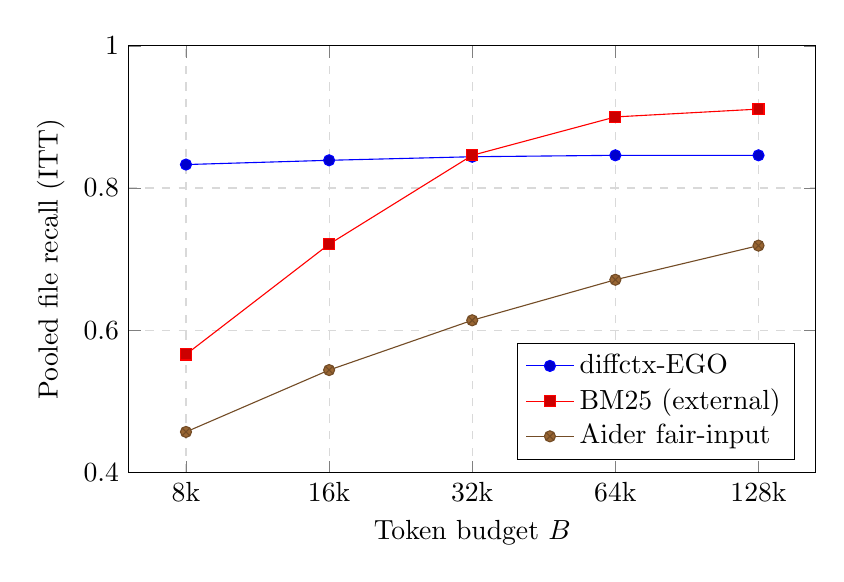
\begin{tikzpicture}
\begin{axis}[
    width=0.85\textwidth, height=7cm,
    xmode=log, log basis x=2,
    xlabel={Token budget $B$}, ylabel={Pooled file recall (ITT)},
    xtick={8000,16000,32000,64000,128000},
    xticklabels={8k,16k,32k,64k,128k},
    ymin=0.4, ymax=1.0,
    legend pos=south east, legend cell align=left,
    grid=major, grid style={dashed,gray!30},
]
\addplot coordinates {(8000,0.833) (16000,0.839) (32000,0.844) (64000,0.846) (128000,0.846)};
\addlegendentry{diffctx-EGO}
\addplot coordinates {(8000,0.566) (16000,0.721) (32000,0.846) (64000,0.900) (128000,0.911)};
\addlegendentry{BM25 (external)}
\addplot coordinates {(8000,0.457) (16000,0.544) (32000,0.614) (64000,0.671) (128000,0.719)};
\addlegendentry{Aider fair-input}
\end{axis}
\end{tikzpicture}
\caption{Pooled file recall vs.\ token budget (intent-to-treat, $n{=}1500$). diffctx-EGO is nearly flat---$0.833$ at $B{=}8000$ already---while whole-file BM25 packing needs ${\sim}32\mathrm{k}$ tokens to catch up and Aider trails at every budget; the whole-system advantage over external whole-file baselines is specific to the tight-budget regime. Data from Tables~\ref{tab:prelim-budget}--\ref{tab:bm25-budget-curve}.}
\label{fig:budget-curves}
\end{figure}

For comparison, Table~\ref{tab:aider-budget-curve} reports the same budget sweep for the Aider repo-map fair-input baseline. The $16\times$ budget gap between the two protocols at the headline crossover is informative: diffctx-EGO at $B{=}8000$ achieves pooled recall $0.833$, while Aider at $B{=}128{,}000$ reaches only $0.719$; the lexical/structural primitives Aider's repo-map builds on do not appear to compensate for the absence of typed-edge propagation even when granted an order-of-magnitude larger token budget.

\begin{table}[h]
\centering
\small
\caption{Budget curve for the Aider repo-map fair-input baseline at the same instance-level inputs. Per-benchmark recall and pooled recall with 95\% percentile bootstrap CIs ($B{=}10{,}000$ resamples, seed=42), intent-to-treat over $n{=}500$ per test set ($n{=}1500$ pooled). $B{=}0$ is the recall-floor sanity bound; $B{=}-1$ is excluded as Aider does not accept an unlimited-budget directive.}
\label{tab:aider-budget-curve}
\resizebox{\textwidth}{!}{%
\begin{tabular}{lrllll}
\toprule
\textbf{Budget $B$} & \textbf{n} & \textbf{ContextBench Verified} & \textbf{PolyBench-500} & \textbf{SWE-bench Verified} & \textbf{Pooled} \\
\midrule
$0$         & 1500 & 0.000 & 0.000 & 0.000 & 0.000 \\
$8{,}000$   & 1500 & 0.432 [0.396, 0.468] & 0.284 [0.249, 0.320] & 0.657 [0.617, 0.698] & 0.457 [0.434, 0.481] \\
$16{,}000$  & 1500 & 0.509 [0.474, 0.544] & 0.356 [0.319, 0.394] & 0.766 [0.730, 0.801] & 0.544 [0.521, 0.567] \\
$32{,}000$  & 1500 & 0.601 [0.566, 0.637] & 0.401 [0.363, 0.440] & 0.839 [0.806, 0.869] & 0.614 [0.591, 0.636] \\
$64{,}000$  & 1500 & 0.662 [0.627, 0.696] & 0.455 [0.416, 0.495] & 0.897 [0.870, 0.921] & 0.671 [0.649, 0.693] \\
$128{,}000$ & 1500 & 0.714 [0.680, 0.747] & 0.527 [0.489, 0.566] & 0.916 [0.892, 0.938] & 0.719 [0.698, 0.739] \\
\bottomrule
\end{tabular}}
\end{table}

The same sweep for the external BM25 baseline (Table~\ref{tab:bm25-budget-curve}) bounds the regime in which graph-based selection helps: whole-file lexical packing is far behind at tight budgets ($0.566$ vs.\ $0.833$ pooled at $B{=}8000$) but overtakes diffctx-EGO once the budget is large enough to simply include most candidate files---pooled $0.846$ vs.\ $0.844$ at $B{=}32\mathrm{k}$, $0.900$ vs.\ $0.846$ at $64\mathrm{k}$, $0.911$ vs.\ $0.846$ at $128\mathrm{k}$. The whole-system advantage over external whole-file baselines is therefore specific to the tight-budget regime ($B \lesssim 16\mathrm{k}$)---attributing it to the typed graph specifically awaits the internal-BM25 cell of the consolidated rerun---which is exactly the regime motivating the problem (Section~\ref{sec:problem}, cost model and ``lost in the middle''~\cite{liu2023lost}); at large budgets, recall saturates for any reasonable method and precision, not recall, becomes the binding concern.

\begin{table}[h]
\centering
\small
\caption{Budget curve for the external BM25-over-patch-identifiers baseline, same protocol (intent-to-treat, $n{=}500$ per test set). BM25 does not support $B{=}{-1}$ (it packs whole files in rank order to the budget).}
\label{tab:bm25-budget-curve}
\resizebox{\textwidth}{!}{%
\begin{tabular}{lrllll}
\toprule
\textbf{Budget $B$} & \textbf{n} & \textbf{ContextBench Verified} & \textbf{PolyBench-500} & \textbf{SWE-bench Verified} & \textbf{Pooled} \\
\midrule
$0$         & 1500 & 0.000 & 0.000 & 0.000 & 0.000 \\
$8{,}000$   & 1500 & 0.485 & 0.672 & 0.540 & 0.566 \\
$16{,}000$  & 1500 & 0.625 & 0.781 & 0.756 & 0.721 \\
$32{,}000$  & 1500 & 0.737 & 0.871 & 0.931 & 0.846 \\
$64{,}000$  & 1500 & 0.806 & 0.925 & 0.970 & 0.900 \\
$128{,}000$ & 1500 & 0.849 & 0.936 & 0.947 & 0.911 \\
\bottomrule
\end{tabular}}
\end{table}

\subsection{Limitations of the Current Empirical Snapshot}
\label{sec:limitations}

The numbers in this section reflect the v2 sweep at commit \texttt{7458eced}. The following items are honest open questions about the snapshot:

\begin{itemize}
    \item \textbf{SWE-bench Verified file recall is saturated.} On SWE-bench Verified, both graph-based scoring modes (EGO and PPR) return $0.913$ at every budget from $8000$ to the unbounded cap, while external BM25 rises from $0.540$ at $B{=}8000$ to $0.970$ at $64\mathrm{k}$ and then dips to $0.947$ at $128\mathrm{k}$ (a pack-order non-monotonicity of skip-and-continue file packing, Table~\ref{tab:bm25-budget-curve}). The plateau is structural: SWE-bench Verified ships no context annotation, so $G = \mathrm{files}(\Delta)$ by construction (Section~\ref{sec:eval}) and recall measures seed retention only; the residual gap to $1.0$ is \emph{hypothesized} to be seed loss inside the pipeline (filtering or oversized-file handling of patch files)---an engineering property rather than a scoring one---pending a per-instance accounting of the missing gold files from the consolidated rerun's logs, which now record the selected file set per instance. SWE-bench Verified is therefore informative as a baseline-comparison metric (graph $\gg$ lexical at small budgets) but uninformative as a scoring-mode comparison.
    \item \textbf{PolyBench-500 fragment-level metrics are not reported.} PolyBench-500 ships a \texttt{modified\_nodes} field encoding CST node paths (e.g., \texttt{file.java->program->class\_declaration:Foo->method\_declaration:bar}) rather than line ranges, and the current adapter does not yet resolve these symbolic paths to \texttt{(start\_line, end\_line)} tuples via a tree-sitter pass on the post-patch worktree. PolyBench-500 therefore contributes to file-level recall only; fragment-level and line-level metrics on this benchmark are deferred.
    \item \textbf{Aider PolyBench-500 infrastructure failure rate.} Aider fair-input on PolyBench-500 has a $24.4\%$ non-\texttt{ok} status rate at $B{=}8000$: $85$ instances ($17.0\%$) hit the $600$s helper-process timeout, and $37$ instances ($7.4\%$) fail with \texttt{QueryError: Invalid node type at row 2, column 2: module} — a tree-sitter grammar version mismatch in the bundled \texttt{aider-chat==0.86.2} package against the installed parsers. The intent-to-treat number ($0.284$ pooled at $B{=}8000$) folds these failures in as recall $0$; an \emph{ok}-only sensitivity analysis on the same cells gives $0.375$ on PolyBench-500, still well below external BM25 ($0.673$ on the same instances). For comparison, Aider's \texttt{ok\%} is $94.0\%$ on SWE-bench Verified (mostly Python, the language Aider's repo-map heuristics are most mature on) and $84.8\%$ on ContextBench Verified. The Aider oracle-mentioned variant (\texttt{mentioned\_fnames} populated from \texttt{instance.gold\_files}, an upper-bound stress test rather than a baseline) is part of the consolidated rerun; whether Aider-oracle approaches diffctx-EGO recall is the open question.
    \item \textbf{$(\tau, \beta_{\mathrm{core}})$ post-fix re-calibration.} The hyperparameter calibration in Section~\ref{sec:greedy} predates the seed/selection fixes that produced the v2 numbers (in particular the rescue pass for cores skipped from $\beta_{\mathrm{core}}\cdot B$ and the inclusion of pure-rename new paths in the candidate set). A focused re-calibration sweep over $\tau \in \{0.04, 0.08, 0.12, 0.16, 0.20\}$ on the v2 pipeline is scheduled; we expect the surface to remain flat as in v1 (Table~\ref{tab:calibration-grid}), but report the v2 calibration as an open item rather than relying on the v1 result.
    \item \textbf{Go out-of-memory class.} 21 of 40 Go instances are killed out-of-memory during graph construction on large vendored-dependency repositories and score recall $0$ under intent-to-treat (Section observations above). Bounding peak memory of edge materialization (currently up to millions of candidate edges before the per-source cap) is the open engineering item; until fixed, Go ITT numbers measure infrastructure, not retrieval.
    \item \textbf{Promised ablations not yet run.} Two ablations referenced by the methodology are open: objective-level (submodular concept coverage vs.\ modular relevance at matched budgets, Section~\ref{sec:utility}) and stopping (with vs.\ without adaptive stopping at matched budgets, Section~\ref{sec:greedy}). The clean-run flags (\texttt{DIFFCTX\_OBJECTIVE}, \texttt{DIFFCTX\_RELATEDNESS\_BONUS}, \texttt{DIFFCTX\_EGO\_LEXICAL\_EPS}) exist so both can be run without pipeline code changes; stopping is disabled via \texttt{-{}-tau 0} (no dedicated flag). The sweep harness does not yet expose these variables as sweep axes---that is orchestration work for the consolidated rerun, alongside an internal-BM25 cell, a changed-files-only floor baseline, and random/degree-matched scoring floors.
    \item \textbf{Per-future timeout.} The runner's per-future timeout does not enforce in single-worker mode because \texttt{concurrent.futures.as\_completed} applies a bulk deadline rather than per-call. About 2\% of instances exceed the configured 180\,s; this increases wall-clock but does not corrupt results.
    \item \textbf{Patch-apply failures were not status-gated at the sweep commit.} At \texttt{7458eced} the eval harness called \texttt{apply\_as\_commit} without checking its return value, so instances whose gold patch failed \texttt{git apply --index} were silently scored against an unrelated diff (the base commit's own history) rather than excluded as the docstring contract specified. Fixed post-snapshot (commit \texttt{7711da24}) to record \texttt{status=apply\_fail} and exclude from metrics, matching \texttt{clone\_fail}. Re-measuring on the same manifests with the fix shows the exposure is small and dataset-driven: $5/500$ ($1.0\%$) on PolyBench-500, $0/500$ on ContextBench Verified and SWE-bench Verified, pooled $\approx 0.33\%$, the same five instances regardless of scoring mode (consistent with a revision-pin issue in those five gold patches, not a scoring-mode effect). Because an unrelated diff rarely overlaps the true gold set, these instances almost certainly already contributed recall $\approx 0$ under the pre-fix code; the bound on the resulting shift in pooled recall is well inside the reported CI half-width ($\pm 0.017$), so the headline numbers are not expected to change materially. A full re-run with the fix is recorded as an open item for the next revision rather than performed retroactively on this snapshot.
\end{itemize}

\newpage
\section{Discussion and Limitations}

\paragraph{Language Coverage.}
The framework requires language-specific tooling for AST parsing and name resolution. Coverage follows the taxonomy of Appendix~\ref{sec:impl-inventory} (Table~\ref{tab:language-support}): structural parsing for $\approx$40 formats; 36 dedicated semantic edge-builder modules (a module may cover several languages) plus a separate config-edge family; structural fragmentation without semantic edges for the remainder; and empirical validation ($n \geq 10$ evaluation instances) for eight languages only (Python, TypeScript, JavaScript, Java, Go, C, Rust, C++). Everything outside that validated tier is a code-level claim, not an empirical one. Dynamic languages present challenges due to incomplete static analysis of dynamic dispatch.

\paragraph{Symbol Reference vs. Data-Flow.}
Our ``symbol reference'' edges use lexical name matching within function scope as a heuristic. This is \textbf{not} true data-flow analysis, which requires CFG construction and reaching definitions computation---infeasible for incomplete code in git working trees. We explicitly acknowledge this limitation.

\paragraph{Forward-Backward PPR Sensitivity.}
The implementation runs PPR on both the original graph and its transpose and linearly blends the two scores (Equation~\ref{eq:ppr-blend}); for change-understanding the default is backward-leaning ($\rho{=}0.4$). The blend weight $\rho$ has not been re-calibrated per language or per benchmark; sensitivity to $\rho$ is a natural extension and is recorded as future work.

\paragraph{Hub Node Dominance.}
Utility classes with high in-degree (Logger, Config, Utils) can accumulate excessive PPR mass. Our implementation applies two mechanisms (Heuristics Annex): IDF-style damping $w'_{uv} = w_{uv} / \log(1 + \text{in\_degree}(v))$ for nodes exceeding the 95th percentile in-degree, and an out-fan mechanism damping \texttt{Semantic} edges from source nodes that reference three or more distinct files ($w / \sqrt{\mathrm{fan}}$). The two do not compose the way the motivation suggests: the in-degree mechanism \emph{exempts} the \texttt{Semantic}, \texttt{Structural}, and \texttt{TestEdge} categories, yet canonical utility hubs accumulate their mass precisely through \texttt{Semantic} call/import edges---so the canonical hub scenario is untouched by in-degree damping and covered only partially by the out-fan rule. The exemption encodes a judgment that structural edges are load-bearing and should not be degree-penalized; whether the net configuration actually suppresses hub dominance is an open empirical question, and a hub-suppression on/off ablation is part of the consolidated sweep.

\paragraph{Configuration Files.}
Non-code files (YAML, JSON, TOML) lack structural dependencies. For these, lexical signals must dominate, with higher BM25 weights (0.4--0.5).

\paragraph{Parameter Sensitivity.}
While we provide operational ranges for parameters ($\alpha$, $\tau$, edge weights), optimal values are repository-dependent. We recommend calibration on 20--50 historical commits via grid search.

\newpage
\section{Conclusion}

We have presented diffctx, a framework for diff-aware code context selection that formulates the problem as budgeted utility maximization over multi-resolution fragments on a typed dependency graph. The deployed system maximizes a monotone submodular concept-coverage objective with lazy-greedy budgeted selection and engineering heuristics, including an adaptive stopping rule that carries an additive loss certificate (Proposition~\ref{prop:stopping}). A pluggable scoring abstraction (EGO, PPR, BM25) allows the same selection algorithm to be instantiated with different relevance signals without changing the optimization machinery; bounded ego-network expansion (EGO) is the deployed default, motivated empirically by the ablation in Section~\ref{sec:prelim-results}. We do not claim a new approximation algorithm; we use known optimization structure to make context selection explicit, analyzable, and extensible.

Key contributions: (1) an explicit ``algorithm $\times$ constraint $\times$ guarantee'' map (Table~\ref{tab:algo-constraint-guarantee}) that separates the deployed heuristic from analyzable variants of the framework, with the submodular concept-coverage objective (Section~\ref{sec:utility}) as the deployed default and the modular Boltzmann variant as opt-in; (2) a typed-edge dependency graph with per-category treatment (hub-suppression exemption for semantic, structural, and test edges); (3) empirical results (Section~\ref{sec:prelim-results}) showing pooled file recall $0.833$ [95\% CI $0.816, 0.850$] at $B{=}8000$ on 1500 multi-language instances under the deployed-default EGO scoring mode (per-benchmark recall: SWE-bench Verified $0.913$, PolyBench-500 $0.847$, ContextBench Verified $0.739$), and paired-bootstrap comparisons against two same-budget baselines: against external BM25-over-patch-identifiers, pooled $\Delta = +0.267$ [$+0.245, +0.290$], one-sided Wilcoxon $p < 2.2\times10^{-16}$; against Aider repo-map (fair-input mode), pooled $\Delta = +0.376$ [$+0.348, +0.403$], $p < 2.2\times10^{-16}$ ($n{=}1500$ in both). The Aider budget curve (Table~\ref{tab:aider-budget-curve}) shows that even at $B{=}128{,}000$ pooled Aider recall reaches only $0.719$, below the diffctx-EGO recall of $0.833$ at the $16\times$ smaller $B{=}8000$ budget. We further report a scoring-mode ablation (EGO, PPR, external BM25 reference at $B{=}8000$) showing EGO $\geq$ PPR $>$ BM25 with the two graph modes $\approx$26--27 points above the lexical baseline pooled; and a budget curve $B \in \{0, 8\mathrm{k}, 16\mathrm{k}, 32\mathrm{k}, 64\mathrm{k}, 128\mathrm{k}, -1\}$ showing recall reaches $0.833$ at $B{=}8000$ and saturates by $B{=}128\mathrm{k}$ (heuristic-bounded asymptote $0.855$ at the unbounded token cap $B{=}{-1}$). Conversely, whole-file BM25 packing overtakes EGO beyond ${\sim}32\mathrm{k}$ tokens (Table~\ref{tab:bm25-budget-curve}), scoping the contribution to the tight-budget regime in which context selection is actually hard.

\subsection{Future Work}
\label{sec:future-work}

\paragraph{Additional behavioral proxies.} The current evaluation uses file-level recall against an annotated golden set. Three complementary proxies are natural extensions:
\begin{itemize}
    \item \textbf{Dependency coverage recall.} For a diff $\Delta$, define $\mathrm{Coverage}(C, \Delta) = |\{d \in \mathrm{deps}(\Delta) : \exists f \in C, d \text{ resolves in } f\}| / |\mathrm{deps}(\Delta)|$, where $\mathrm{deps}(\Delta)$ is the set of definitions of modified symbols, call targets, callers, types in signatures, and covering tests. This complements file recall by measuring whether the selected context resolves the symbols that appear in the diff~\cite{parnin2011automated}.
    \item \textbf{Co-change recall.} For commits where files $A$ and $B$ change together, input only $A$'s diff and measure whether $B$ appears in $C$. Co-change has a 30--40\% incidental-coupling false-positive rate~\cite{hassan2004predicting}; the proxy is meaningful only after filtering to semantic modifications ($\geq 5$ substantive lines).
    \item \textbf{Fault-localization accuracy.} Given $(\Delta, C)$, an LLM-based or human evaluator ranks suspicious lines for root-cause identification, scored by Mean Reciprocal Rank and Precision@$k$~\cite{parnin2011automated}.
\end{itemize}

\paragraph{Edge-weight calibration on labeled corpora.} Section~\ref{sec:weight-calibration} fixes $w_t$ at author-selected priors informed by the code-navigation literature. A larger labeled corpus (e.g., a sweep across all six benchmarks combined) would enable the full $|T|$-dimensional calibration of $w_t$, with the formulation already laid out there. Richer parameterizations (per-edge MLP over edge-context features) become tractable once labeled data scales further.

\paragraph{Blend sensitivity, memory, and dynamic dispatch.} Forward--backward PPR blending is already deployed (Equation~\ref{eq:ppr-blend}, $\rho = 0.4$); per-language and per-benchmark sensitivity to $\rho$ has not been studied and is a direct extension. The most acute engineering item is the Go out-of-memory class (Section~\ref{sec:limitations}): bounding peak memory of edge materialization would recover the 21 currently-failing Go instances whose completed peers score $0.935$. Per-language semantic resolvers (e.g.\ for interface-method-set dispatch and metaprogramming-heavy code) remain valuable for the residual gap between dynamic and statically-typed languages on completed instances.

\newpage
\section*{Acknowledgments}

The reference implementation lives at \url{https://github.com/nikolay-e/diffctx}.

\appendix

\newpage
\section{Parameter Guidelines}

\begin{table}[h]
\centering
\begin{tabular}{llp{6cm}}
\toprule
\textbf{Parameter} & \textbf{Range} & \textbf{Selection Guidance} \\
\midrule
$\alpha$ (damping) & 0.50--0.65 & Start at 0.60; decrease for over-selection of distant code \\
$\tau$ (threshold) & 0.04--0.16 (grid) & Deployed calibrated default 0.12; 0.08 is an uncalibrated heuristic for narrowly-scoped fixes \\
Budget $B$ & 5k--20k tokens & 10k standard; scale with diff complexity \\
Call weight & 0.65--0.75 & Matches \texttt{config/weights.rs} (Section~\ref{sec:weight-calibration}); tune via cross-validation on historical commits \\
Lexical weight & 0.1--0.2 & Reduce if high false positive rate \\
Overhead & 15--20 tokens & Measure actual serialization cost per fragment \\
\bottomrule
\end{tabular}
\caption{Operational parameter ranges with selection heuristics.}
\end{table}

\paragraph{Implementation parameters not modelled in Section~\ref{sec:problem}--\ref{sec:greedy}.} The reference implementation exposes additional parameters that govern second-order behaviors not formalized in the body: a relevance-augmentation weight \texttt{UtilityConfig.eta} ($0.20$) blending raw PPR scores into match strength; a structural-bonus weight \texttt{UtilityConfig.structural\_bonus\_weight} ($0.10$) adding a small bonus when a fragment has any matched need; an $r_{\mathrm{cap}}$ calibration constant \texttt{UtilityConfig.r\_cap\_sigma} ($2.0$, in standard deviations) controlling the soft cap on per-fragment relevance contribution; a hunk-proximity decay system (\texttt{FilteringConfig.proximity\_half\_decay} = $50$ lines, \texttt{FilteringConfig.definition\_proximity\_half\_decay} = $5$ lines, \texttt{UtilityConfig.proximity\_decay} = $0.30$) that boosts fragments physically near diff hunks; BM25 hyperparameters \texttt{Bm25Config.idf\_smoothing} ($0.5$) and \texttt{Bm25Config.min\_query\_token\_length} ($3$), with the average document length computed from the corpus; the Boltzmann calibration loop's bisection bounds \texttt{BoltzmannConfig.beta\_lo} ($10^{-6}$), \texttt{BoltzmannConfig.beta\_hi} ($1.0$), iteration cap \texttt{BoltzmannConfig.bisect\_iters} ($24$), and convergence tolerance \texttt{BoltzmannConfig.calibration\_tolerance} ($5\%$ of budget); and the rescue-phase parameters \texttt{RescueConfig.budget\_fraction} ($0.05$) and \texttt{RescueConfig.min\_score\_percentile} ($0.80$). These parameters are calibrated empirically on representative corpora and held fixed across modes; their role is operational rather than theoretical, so we do not model them in the body but document them here for reproducibility.

\newpage
\section{Algorithmic Complexity}

\begin{table}[h]
\centering
\small
\begin{tabular}{p{3.6cm}p{5.2cm}lp{3.4cm}}
\toprule
\textbf{Component} & \textbf{Time} & \textbf{Space} & \textbf{Practical Scale} \\
\midrule
AST parsing & $O(n)$ & $O(n)$ & Tested to $\sim$500k LOC \\
Semantic/structural edge builders & $O(n \log n)$ & $O(n+m)$ & Tested to $\sim$200k LOC \\
Similarity (TF--IDF) edges & $O(n \cdot \bar{t})$, $\bar{t}$ = tokens per fragment & $O(n+m)$ & --- \\
History (co-change) edges & $O(h)$, $h$ = git-log entries & $O(m)$ & --- \\
PPR (forward-push) & $O(\mathrm{pushes})$, cap $\min(100n,\,2{\times}10^6)$ & $O(n+m)$ & Tested to $\sim$50k nodes \\
Lazy greedy & $O(|\mathcal{V}| \log |\mathcal{V}|)$ typical; $O(|\mathcal{V}|^2)$ recomputations worst case & $O(n)$ & Tested to $\sim$5k fragments \\
Post-passes & $O(|C| \cdot \bar{d} + n)$ & $O(n)$ & Bounded by remaining budget \\
\bottomrule
\end{tabular}
\caption{Complexity analysis where $n$ = fragments, $m$ = edges, $\bar{d}$ = average degree. PPR uses a forward-push (local-push) solver with a global push cap, not power iteration, so its cost is measured in pushes rather than iteration count. Practical scale limits are estimates requiring validation; performance depends on repository structure and hardware. Empirical run-time and memory telemetry (p50/p90/p99 per-instance latency, peak RSS, node/edge counters, per-phase shares, timeout/OOM rates) is collected per instance by the harness and will be reported from the consolidated rerun's logs.}
\end{table}

\newpage
\section{Heuristics Annex}

The following tactics are useful in practice but lack strong theoretical or empirical grounding. They should be evaluated via ablation before deployment.

\paragraph{Relatedness (Diversity) Bonus.} Fragments with relevance above a small threshold ($\geq 0.03$, \texttt{NeedsConfig.min\_rel\_for\_bonus}) receive an additional marginal gain $\text{rel} \times 0.25 \times \text{unsatisfied}(C)$, where $\text{unsatisfied}(C) = \max(0,\, 1 - \sum_z \mathrm{cov}_z(C)/|Z|)$ is the fraction of concept mass not yet covered by the selected set. This keeps structurally related fragments in play early while fading the bonus as coverage saturates. Separately, a modular structural bonus of $0.10 \cdot r_{\mathrm{norm}}$ applies to fragments matching at least one need (\texttt{UtilityConfig.structural\_bonus\_weight}). \textbf{Warning:} the diversity term is path-dependent (its increment depends on coverage at selection time) and falls outside the strict set-function form, so worst-case approximation guarantees do not apply to the deployed configuration; its increment is pointwise non-increasing in $C$, which is the property Proposition~\ref{prop:stopping} needs. Setting \texttt{DIFFCTX\_RELATEDNESS\_BONUS=0} disables it. An ablation with vs.\ without the bonus is still required.

\paragraph{Hub Suppression.} Apply IDF-style penalty to edges into high in-degree nodes: $w'_{uv} = w_{uv} / \log(1 + \text{in\_degree}(v))$ when $\text{in\_degree}(v)$ exceeds the 95th percentile; edges in the exempt categories (\texttt{Semantic}, \texttt{Structural}, \texttt{TestEdge}) are not damped by this in-degree mechanism. A second, out-fan mechanism damps \texttt{Semantic} edges from source nodes referencing $\geq 3$ distinct files: $w' = w / \sqrt{\mathrm{fan}}$, targeting broad-capture import hubs. Both are implemented globally during graph construction, before the per-source top-$K$ cap.

\paragraph{Backward Edge Weighting.} Weight caller$\to$callee edges at 0.7--0.8$\times$ of callee$\to$caller edges to prioritize impact analysis over dependency tracing.

\paragraph{Test File Handling.} Test-to-code edges are static: direct links (test imports/references the unit) carry weight $0.60$, naming-convention links $0.50$, and reverse (code$\to$test) links $0.30$ (\texttt{config/weights.rs}). The system does not execute tests; upweighting tests that fail after $\Delta$ (e.g.\ to $0.9$) requires runtime signal and is future work.

\paragraph{Signature Variants.} Selection is fragment-granular, so partial function bodies never appear; instead, every full semantic unit gets a signature-only companion fragment (bracket-balanced signature extent, falling back to the first two lines; \texttt{signatures.rs}) that serves as its compact matroid representative when the full body does not fit.

\paragraph{Post-Passes.} After the main greedy loop terminates (either by exhausting the budget or by adaptive stopping, Section~\ref{sec:greedy}), three ordered post-passes run (\texttt{postpass.rs}, \texttt{pipeline.rs}): (i) a \emph{coherence pass} (\texttt{coherence\_post\_pass}) scans the selected set for dangling references---selected fragments whose semantic-neighbor definitions are absent from the context---and pulls in the missing definitions against the full remaining budget; (ii) a \emph{rescue pass} (\texttt{rescue\_nontrivial\_context}) spends a reserved fraction (5\% of $B$, \texttt{RescueConfig.budget\_fraction}) on high-relevance fragments from files not yet represented, gated by a percentile threshold on relevance (\texttt{RescueConfig.min\_score\_percentile} $= 0.80$) so it does not flood the context with low-confidence rescues; (iii) a \emph{changed-files pass} (\texttt{ensure\_changed\_files\_represented}) ensures, budget permitting, that every file touched by $\Delta$ appears at least as a compact representative---adding without any relevance gate (it synthesizes a whole-file fragment if the file has none), but strictly within the remaining budget: when no representative of a changed file fits, the file stays unrepresented and the shortfall surfaces as changed-file retention $<1$ rather than as a budget overrun. All three passes respect $\mathrm{cost}(C) \leq B$ and pairwise-overlap feasibility; for a monotone objective they never decrease utility below the greedy value, but they relax the strict density-greedy ordering, and the rescue and changed-files passes draw candidates from the pre-filter fragment universe, outside the scope of Proposition~\ref{prop:stopping}'s certificate (the coherence pass draws from the post-filter universe and stays within it).

\newpage
\section{Language Support}
\label{sec:impl-inventory}

Two independent layers make up language support, and they are counted separately because neither is a subset of the other. \emph{Structural parsing} (fragmentation): 39 registered tree-sitter grammar keys (38 distinct grammars; JSX aliases the JavaScript grammar) plus a regex-structural TOML splitter and a heading-based Markdown splitter --- about 40 structurally parsed formats. \emph{Semantic edge extraction}: 36 dedicated edge-builder \emph{modules} (excluding one generic cross-file identifier linker), where a single module may cover several languages (one JVM builder serves Java/Kotlin/Scala/Groovy; one C-family builder serves C/C++/Objective-C; the JavaScript builder also serves TypeScript), so the tier rows below enumerate \emph{languages} and legitimately exceed 36. Three builders (LaTeX, Perl, Nim) operate on generically fragmented text without a dedicated parser --- edge building keys off file extension and raw text, not the parse tree. A separate family of six \emph{config} edge builders (Dockerfile, Kubernetes, Helm, CI/CD pipelines, build systems, generic config$\to$code) emits the \texttt{Config}/\texttt{ConfigGeneric} categories of Table~\ref{tab:edge-categories}; the domain builders listed in Tier 2 (Ansible, dbt, OpenAPI, Cargo) sit on generic serialization formats at the parsing layer but re-parse raw text with dedicated extractors and emit \texttt{Semantic} edges. Coverage is uneven: a handful of languages have been exercised extensively in the evaluation; the rest are code-level claims. Table~\ref{tab:language-support} groups by tier of empirical exercise.

\begin{table}[h]
\centering
\small
\begin{tabular}{p{4.2cm}p{10.2cm}}
\toprule
\textbf{Tier} & \textbf{Languages / formats} \\
\midrule
Tier 1 — empirically validated ($n{\geq}10$ in evaluation) &
Python ($n{=}891$), TypeScript ($n{=}191$), JavaScript ($n{=}185$),
Java ($n{=}140$), Go ($n{=}40$), C ($n{=}23$), Rust ($n{=}20$), C++ ($n{=}10$) \\
\midrule
Tier 2 — semantic edge builders, no large-scale empirical validation &
C\#, F\#, VB, Kotlin, Ruby, PHP, Swift, Scala (general-purpose);
Haskell, Elixir, Erlang, OCaml, Clojure, Julia (functional);
Lua, R, Perl, Bash/Zsh/Fish/Ksh, Dart, Groovy, Objective-C, Zig, Nim (scripting/systems);
CSS/SCSS/LESS, GraphQL, HCL/Terraform, Nix, LaTeX (markup/infra);
Cargo, Bazel, dbt, OpenAPI, Prisma, Protobuf, SQL, Ansible (domain; \texttt{Semantic} edges over generic serialization formats) \\
\midrule
Config edge builders (\texttt{Config}/\texttt{ConfigGeneric} categories) &
Dockerfile/Compose, Kubernetes manifests, Helm charts, CI/CD pipelines, build-system files, generic config$\to$code references \\
\midrule
Tier 3 — parser only, structural fragmentation without semantic edges &
YAML, JSON, TOML, Svelte, HTML, CMake, Make (bare files; CMake/Make cross-references are reachable via the build-system config builder) \\
\midrule
Generic fallback &
Markdown (structural heading splitter), plain text, dotfiles, unparsed sources (paragraph or statement fragmentation) \\
\bottomrule
\end{tabular}
\caption{Tiered coverage of the reference implementation. Tier 1 has both edge builders and per-language recall numbers in Table~\ref{tab:prelim-lang}. Tier 2 lists \emph{languages} covered by the 36 dedicated semantic edge-builder modules (a module may serve several languages, so rows exceed 36 by design); its inclusion is a code-level claim, not an empirical one. The config-builder family is a separate edge layer, not a language tier. Tier 3 supplies parsing only. Only Tier 1 carries empirical evidence.}
\label{tab:language-support}
\end{table}

\newpage
\section{Symbol-to-Code Map}
\label{sec:symbol-map}

This appendix records the correspondence between symbols in the body of the paper and their identifiers in the reference Rust implementation. The map is the durable contract between the formalism and the code: a symbol that appears in the paper must resolve to a named field, function, or module in the codebase, and any drift surfaces here. Paths are relative to \texttt{diffctx/src/}.

\begin{table}[h]
\centering
\scriptsize
\resizebox{0.98\textwidth}{!}{%
\begin{tabular}{lp{4.5cm}p{7cm}p{4.2cm}}
\toprule
\textbf{Paper symbol} & \textbf{Meaning} & \textbf{Code identifier} & \textbf{Source} \\
\midrule
$\alpha$            & PPR damping factor             & \texttt{PPRConfig.alpha}                       & \texttt{config/limits.rs} \\
$\rho$              & PPR forward-blend weight (Eq.~\ref{eq:ppr-blend}) & \texttt{PPRConfig.forward\_blend} & \texttt{config/limits.rs} \\
$\beta$             & Boltzmann inverse temperature  & \texttt{BoltzmannConfig.beta\_lo}/\texttt{beta\_hi} (bisection bounds) & \texttt{config/selection.rs} \\
$\beta_{\mathrm{core}}$ & Core edit budget fraction  & \texttt{SelectionConfig.core\_budget\_fraction} & \texttt{config/selection.rs} \\
$\gamma$            & Ego-network per-hop decay (Section~\ref{sec:ego}) & \texttt{EgoScoringConfig.per\_hop\_decay} & \texttt{config/scoring.rs} \\
$\tau$              & Adaptive stopping threshold    & \texttt{DEFAULT\_STOPPING\_THRESHOLD} (CLI \texttt{-{}-tau}) & \texttt{config/limits.rs} \\
$L$                 & Ego-network expansion radius   & \texttt{EgoGraphScoring.max\_depth}            & \texttt{scoring.rs} \\
$k_1$, $b$          & BM25 saturation, length norm   & \texttt{Bm25Config.k1}, \texttt{Bm25Config.b}  & \texttt{config/bm25.rs} \\
$w_t$               & Per-edge-category weight       & \texttt{CategoryWeights.<variant>}             & \texttt{config/category\_weights.rs} \\
$I(f)$              & File-importance prior          & \texttt{utility::importance::compute\_file\_importance} & \texttt{utility/importance.rs} \\
$\omega_f$          & Per-fragment importance scaling & \texttt{compute\_seed\_weights}               & \texttt{core.rs} \\
$E_0$               & Core edit set                  & \texttt{identify\_core\_fragments}             & \texttt{core.rs} \\
$F$                 & Fragment universe              & output of fragment-extraction phase            & \texttt{fragmentation.rs}, \texttt{parsers/} \\
\midrule
\multicolumn{4}{l}{\emph{Pipeline phases:}} \\
File discovery      & Candidate file assembly        & \texttt{candidate\_files::collect\_candidate\_files} & \texttt{candidate\_files.rs} \\
Fragment extraction & Tree-sitter fragmentation      & \texttt{fragmentation::process\_files\_for\_fragments} & \texttt{fragmentation.rs} \\
Symbol-level discovery & Seed expansion via rare idents & \texttt{discovery::*Discovery}              & \texttt{discovery.rs} \\
Scoring             & Pluggable $\hat{w}(f, \Delta)$ & \texttt{PPRScoring}, \texttt{EgoGraphScoring}, \texttt{BM25Scoring} & \texttt{scoring.rs} \\
Filtering           & Relevance/proximity filters    & \texttt{filtering::*}                          & \texttt{filtering.rs} \\
Selection           & Lazy greedy / Boltzmann        & \texttt{select::lazy\_greedy\_select}          & \texttt{select.rs} \\
Coherence post-pass & Rescue dangling references     & \texttt{postpass::coherence\_post\_pass}       & \texttt{postpass.rs} \\
\bottomrule
\end{tabular}}
\caption{Symbol-to-code map. Paper symbols on the left correspond to the named code identifiers on the right, located in the listed source file under \texttt{diffctx/src/}. Implementation-only parameters are documented inline in Appendix~A and are not duplicated here.}
\label{tab:symbol-map}
\end{table}

\bibliographystyle{plain}
\bibliography{references}

\end{document}
